%%%%%%%%%%%%%%%%%%%%%%%%%%%%%%%%%%%%%%%%%%%%%%%%%%%%%%%%%%%%%%%%%%%%%%%%%%%%%%%%
%2345678901234567890123456789012345678901234567890123456789012345678901234567890
%        1         2         3         4         5         6         7         8
% THESIS CHAPTER

% short summary of the chapter
\section*{Summary}
In this chapter we will show the results of classification without the textures and compare it with the results of classification using the additional textures features. It will be shown the results for classification for forest and deforested areas in the Amazon Rain forest looking at acquisitions from the TANDEM-X satellite. Besides that, it will be also shown classification results using the acquisitions of the SENTINEL1 satellite for areas in the Amazon Rain forest, and compare the results with textures and without textures.



\section{TANDEM-X Data Analysis} 
\label{sec:gv2}
On this section it will be analyzed the result of textures for the volumetric correlation of a acquisition of the TANDEM-X satellite. The volumetric correlation image can be seen below.
From this image, the textures were made using the sum and difference histogram method and it was given as a input to a Random Forest algorithm for classification. The random forest was trained using the reference map provided by DLR. Due to computational limitations not all textures were used, but just some of them. The textures choice was based on the PDFs of different classes. The textures chosen as input to the Random Forest algorithms were: Cluster Shade, Cluster Prominence, Contrast, Variance. Besides that, the coherence was also given as an input to the Random Forest Algorithm. The classification results with the textures can be seen below.

\begin{figure}[H]
  \centering
  \begin{subfigure}[b]{0.4\linewidth}
    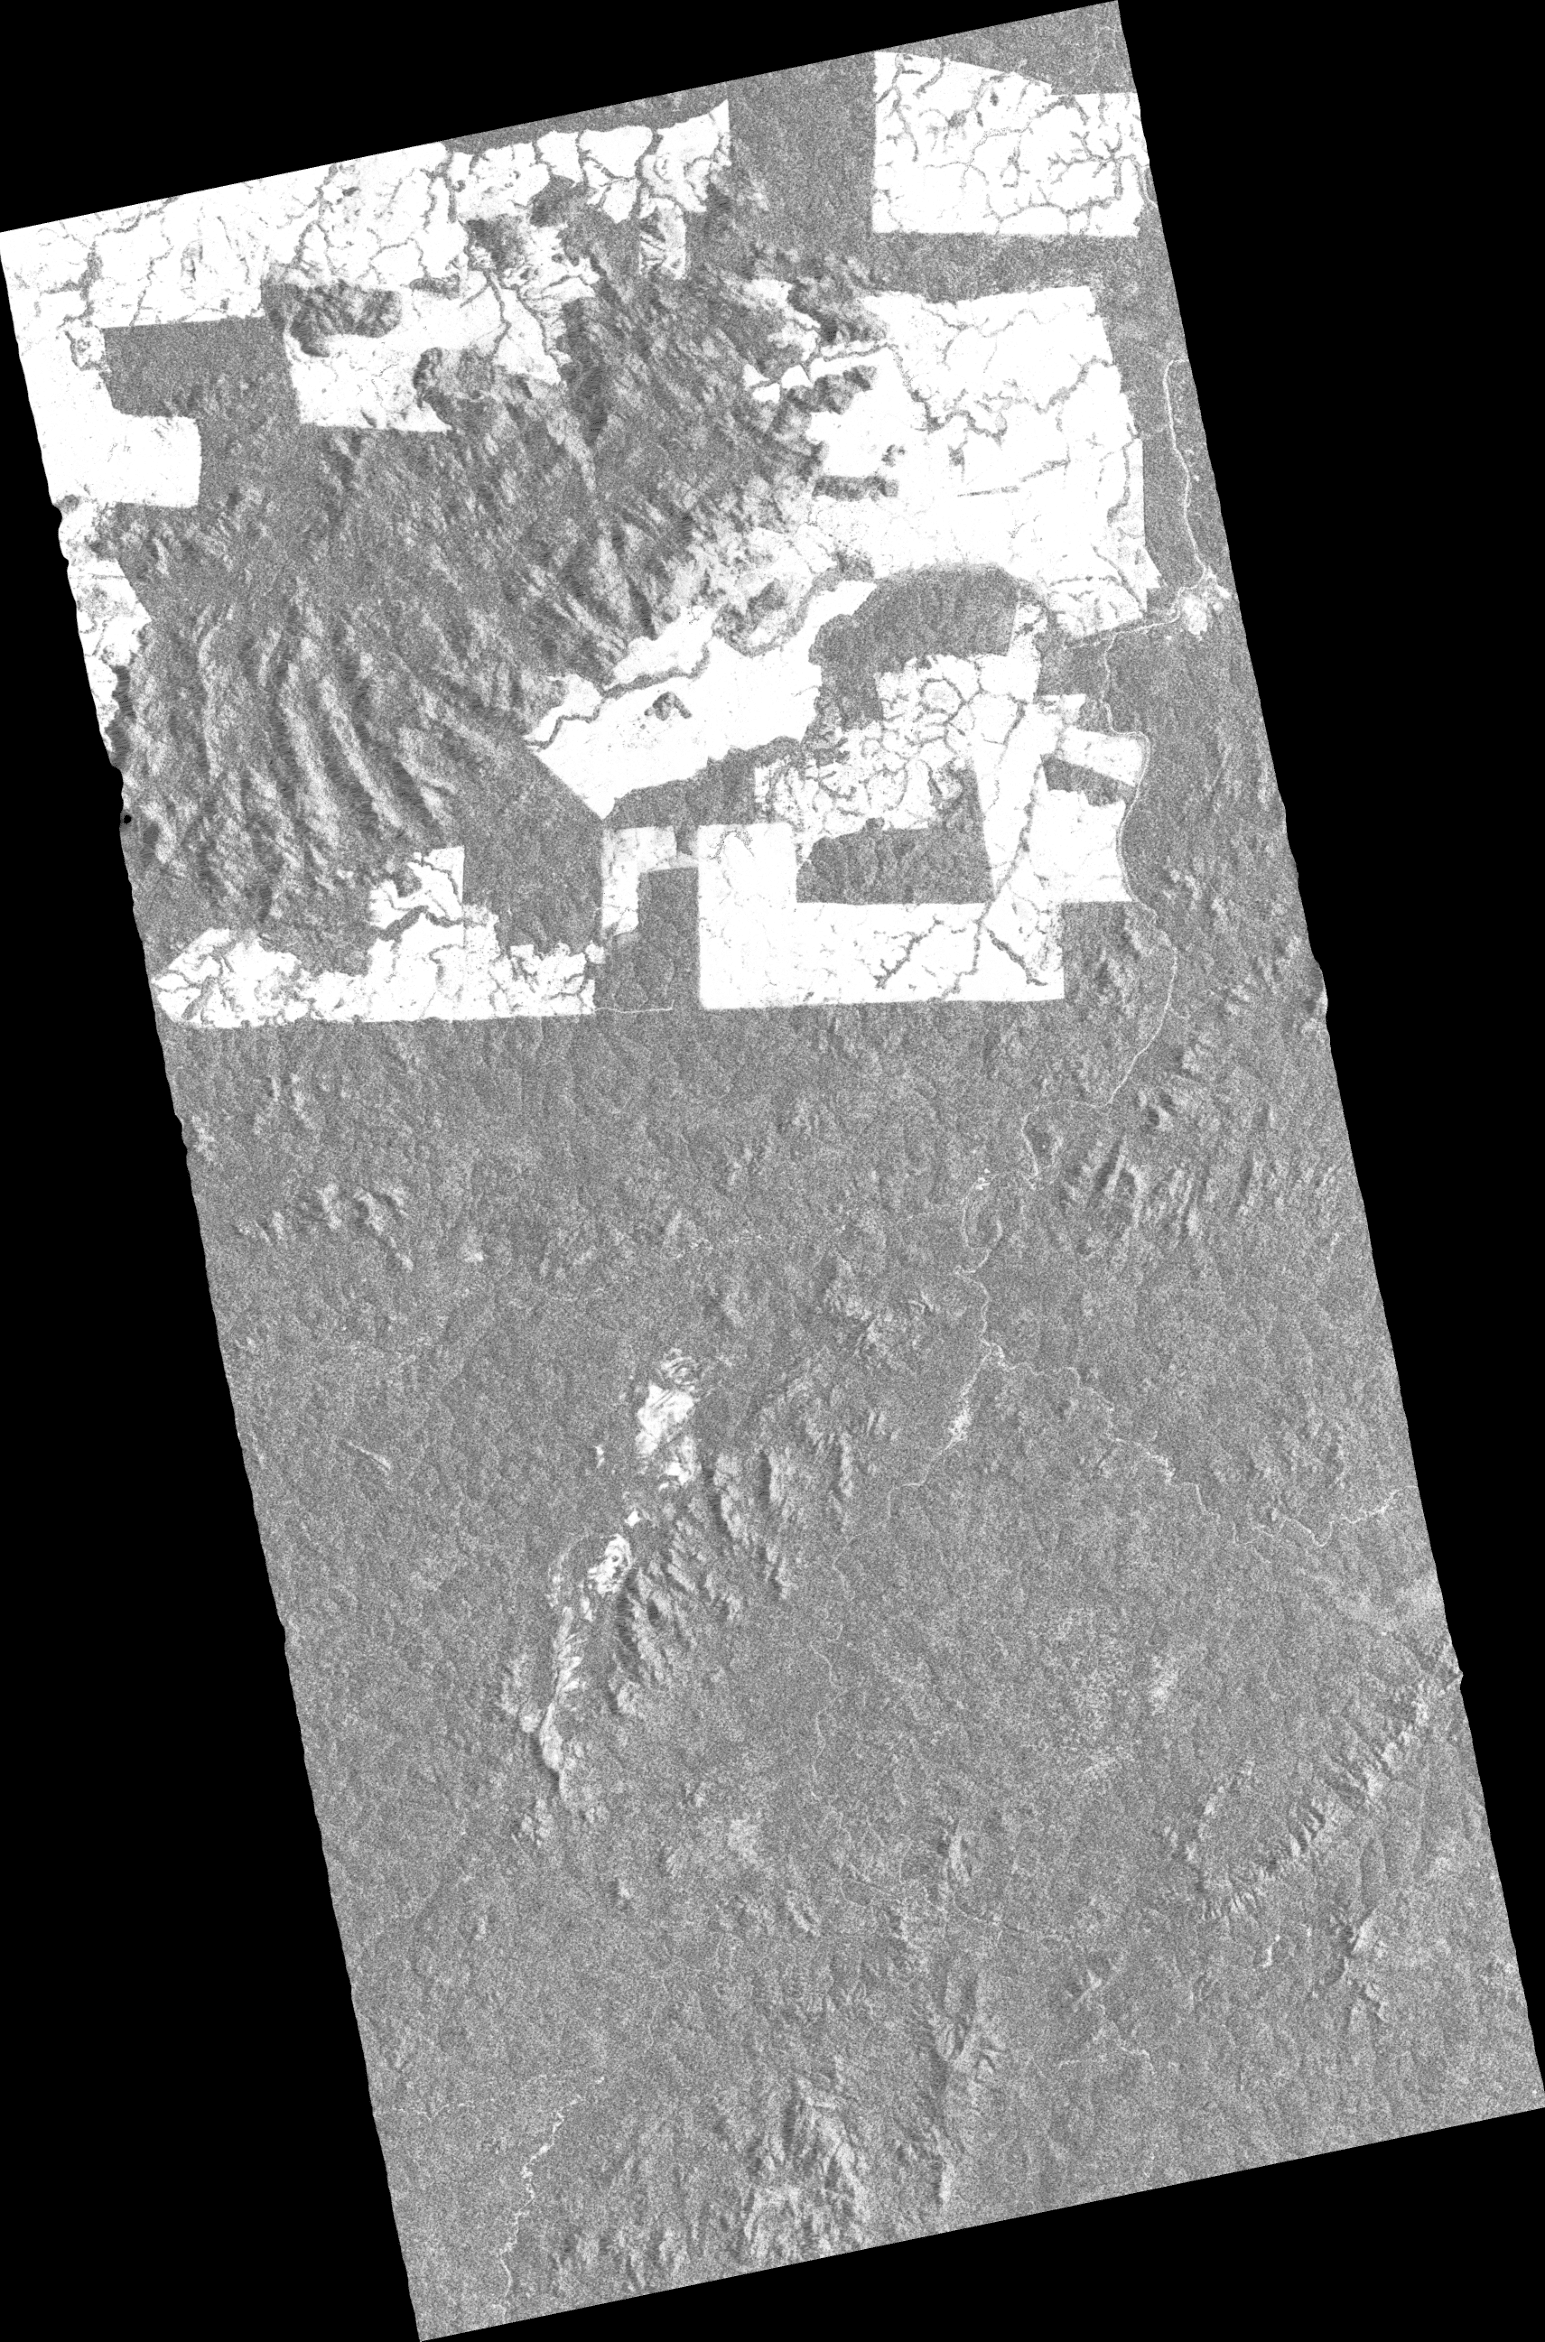
\includegraphics[width=\linewidth]{Chapter5/coSSC_master_gamma_vol.pdf}
     \caption{Volumetric Correlation image of TANDEM-X acquisition}
  \end{subfigure}
  \begin{subfigure}[b]{0.4\linewidth}
    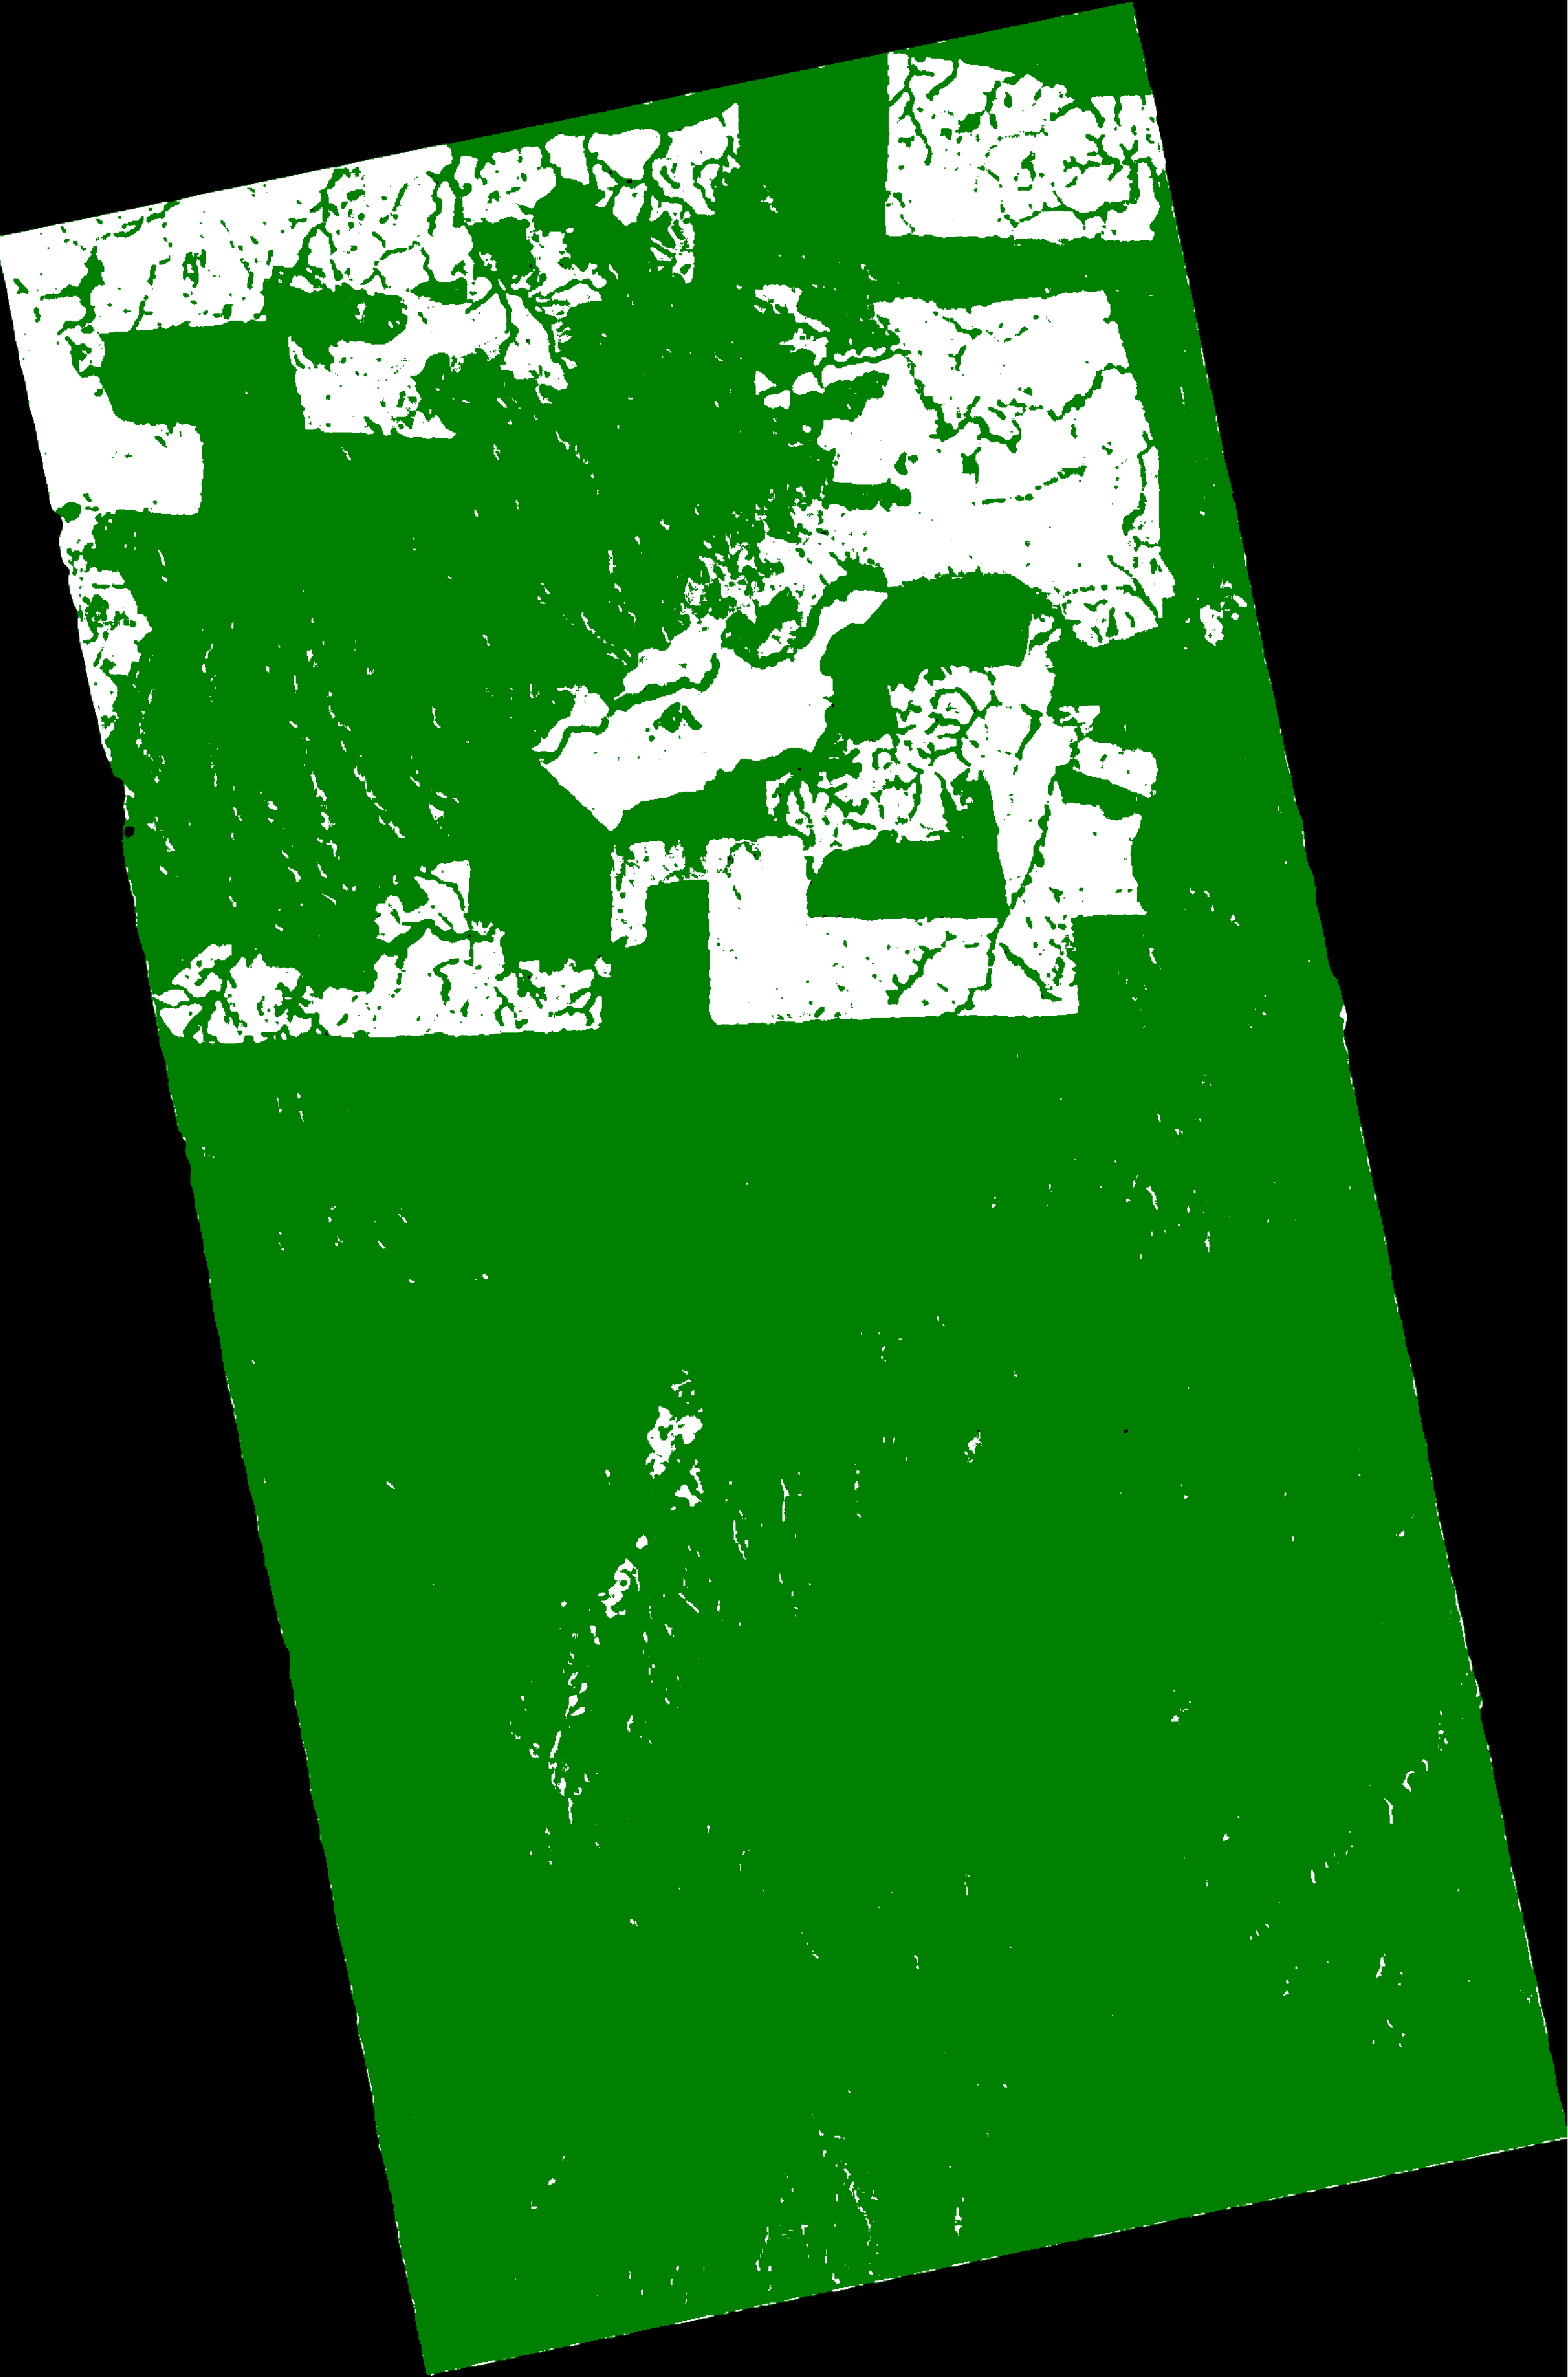
\includegraphics[width=\linewidth]{Chapter5/TANDEM-X/classification_resultsimage.pdf}
    \caption{Random Forest Results with Texture}
  \end{subfigure}
  \caption{Volumetric Correlation and Classification}
  \label{fig:classification_tandem}
\end{figure}

On the volumetric correlation image above the white pixels have higher correlation, which indicate the presence of a deforested area, while the dark pixels have a lower correlation, which is characteristic of a forested area. On the right it is possible to see the classification result given by the random forest. On the classification image on the right the white pixels indicate deforested area while the green pixels indicate the presence of a forested area. \\
It is clear from the figure \ref{fig:classification_tandem} that the classification is accurate, but it is not possible to see how accurate the result is. Due to this it was also obtained the accuracy results when compared to the reference map provided by DLR %\ref{fig:reference_map}
. The accuracy results with different combinations of textures can be seen in the table below

\begin{table}[H]
\centering
\begin{tabular}{ |c |c |}
 \hline
     Variance & 46.78\% \\
     Coherence & 4.70\% \\
     Variance/Coherence & 4.70\% \\
     Cluster Prominence & 3.82\% \\
     Cluster Prominence/Variance & 4.17\% \\
     Cluster Prominence/Coherence & 3.80\% \\
     Cluster Prominence/Variance/Coherence & 4.70\% \\
     Cluster Shade & 1.33\% \\
     Cluster Shade/Variance & 1.30\% \\
     Cluster Shade/Coherence & 1.30\% \\
     Cluster Shade/Variance/Coherence & 1.30\% \\
     Cluster Shade/Cluster Prominence & 1.27\% \\
     Cluster Shade/Cluster Prominence/Variance & 1.26\% \\
     Cluster Shade/Cluster Prominence/Coherence & 1.26\% \\
     Cluster Shade/Cluster Prominence/Variance/Coherence & 1.28\% \\
     Contrast & 21.13\% \\
     Contrast/Variance & 21.07\% \\
     Contrast/Coherence & 5.18\% \\
     Contrast/Variance/Coherence & 4.70\% \\
     Contrast/Cluster Prominence & 4.42\% \\
     Contrast/Cluster Prominence/Variance & 3.81\% \\
     Contrast/Cluster Prominence/Coherence & 3.47\% \\
     Contrast/Cluster Prominence/Variance/Coherence & 3.47\% \\
     Contrast/Cluster Shade & 1.30\% \\
     Contrast/Cluster Shade/Variance & 1.30\% \\
     Contrast/Cluster Shade/Coherence & 1.30\% \\
     Contrast/Cluster Shade/Variance/Coherence & 1.40\% \\
     Contrast/Cluster Shade/Cluster Prominence & 1.15\% \\
     Contrast/Cluster Shade/Cluster Prominence/Variance & 1.52\% \\
     Contrast/Cluster Shade/Cluster Prominence/Coherence & 1.47\% \\
     Contrast/Cluster Shade/Cluster Prominence/Variance/Coherence & 1.29\% \\
 \hline
\end{tabular}
\caption{Error results with different textures combinations}
\label{table:accuracy_results_tandem}
\end{table}

From the table \ref{table:accuracy_results_tandem} we can quantitatively see how much was the improvement. Trying to run a classification using just the Coherence as an input gives a classification error of 4.70\%, while if all textures are used then the error drops to 1.29\%, in a way that the error 3 times smaller than the original error. Keep in mind that the classification map provided by DLR is not 100\% accurate, so these numbers are not 100\% accurate and have a small error, which might explain why using just 2 textures, the cluster shade and cluster prominence, gives a smaller error (1.27\%) than using the 4 textures together with the coherence (1.28\%).

Even though this improvement might seem surprising it is important to notice that the coherence image used was a high quality image acquired with ideal conditions and with a height of ambiguity that yields a clear separation between the forest and deforested areas, but normally the SARs acquisitions are not always this good for classification, specially if it is not used a double satellite system like TANDEM-X (which has the advantage of not having temporal decorrelation between images since they are taken at the same time).
On the next section this method will be used on acquisitions that are not so suited to make a classification in order to see the improvement that the textures can provide in non-ideal conditions.

\section{Sentinel1 Data Analysis}

As said previously, the TANDEM-X images used for classification were taken in ideal conditions, in a way that making a classification on that image only is easy and even if no textures are used the classification results can provide a high accuracy. \newline
The advantage of the TANDEM-X satellite is that it is twin satellite system that fly together taking pictures of the same area at the same time, in a way that the temporal decorrelation does not affect these images. \newline
But normally, the pictures taken with SARs radars are taken at different days, in a way that the temporal changes on the scene strongly affects the image. \newline
To illustrate this, on this section it will be shown coherence images of images of the satellite SENTINEL1, which have a 6 days temporal baseline between acquisitions. There were 5 images that were used to make the classification on this example, taken at the days 25/04/2019, 01/05/2019, 07/05/2019, 13/05/2019/ and 19/05/2019. Due to computational limitations it was chosen to make the mean between the images, since making the textures of each image might take a long time. The images have a 12m pixel resolution and cover an area of almost $40000km^2$, so making the textures of each image can take until 50 hours. \newline
From the acquisitions it is possible to extract the brightness ($\sigma^0)$ of the scene and since there are 5 images it is possible to get 4 coherence images with a 6 days temporal baseline. Even though it is also possible to get the coherence at 12, 18 and 24 days it was chosen not to do so, since the images with such temporal baseline will provide little to no useful information for classification.
Below there are images of the average $\sigma^0$ and the average coherence $\gamma$ of the acquisitions.
\begin{figure}[H]
    \centering
    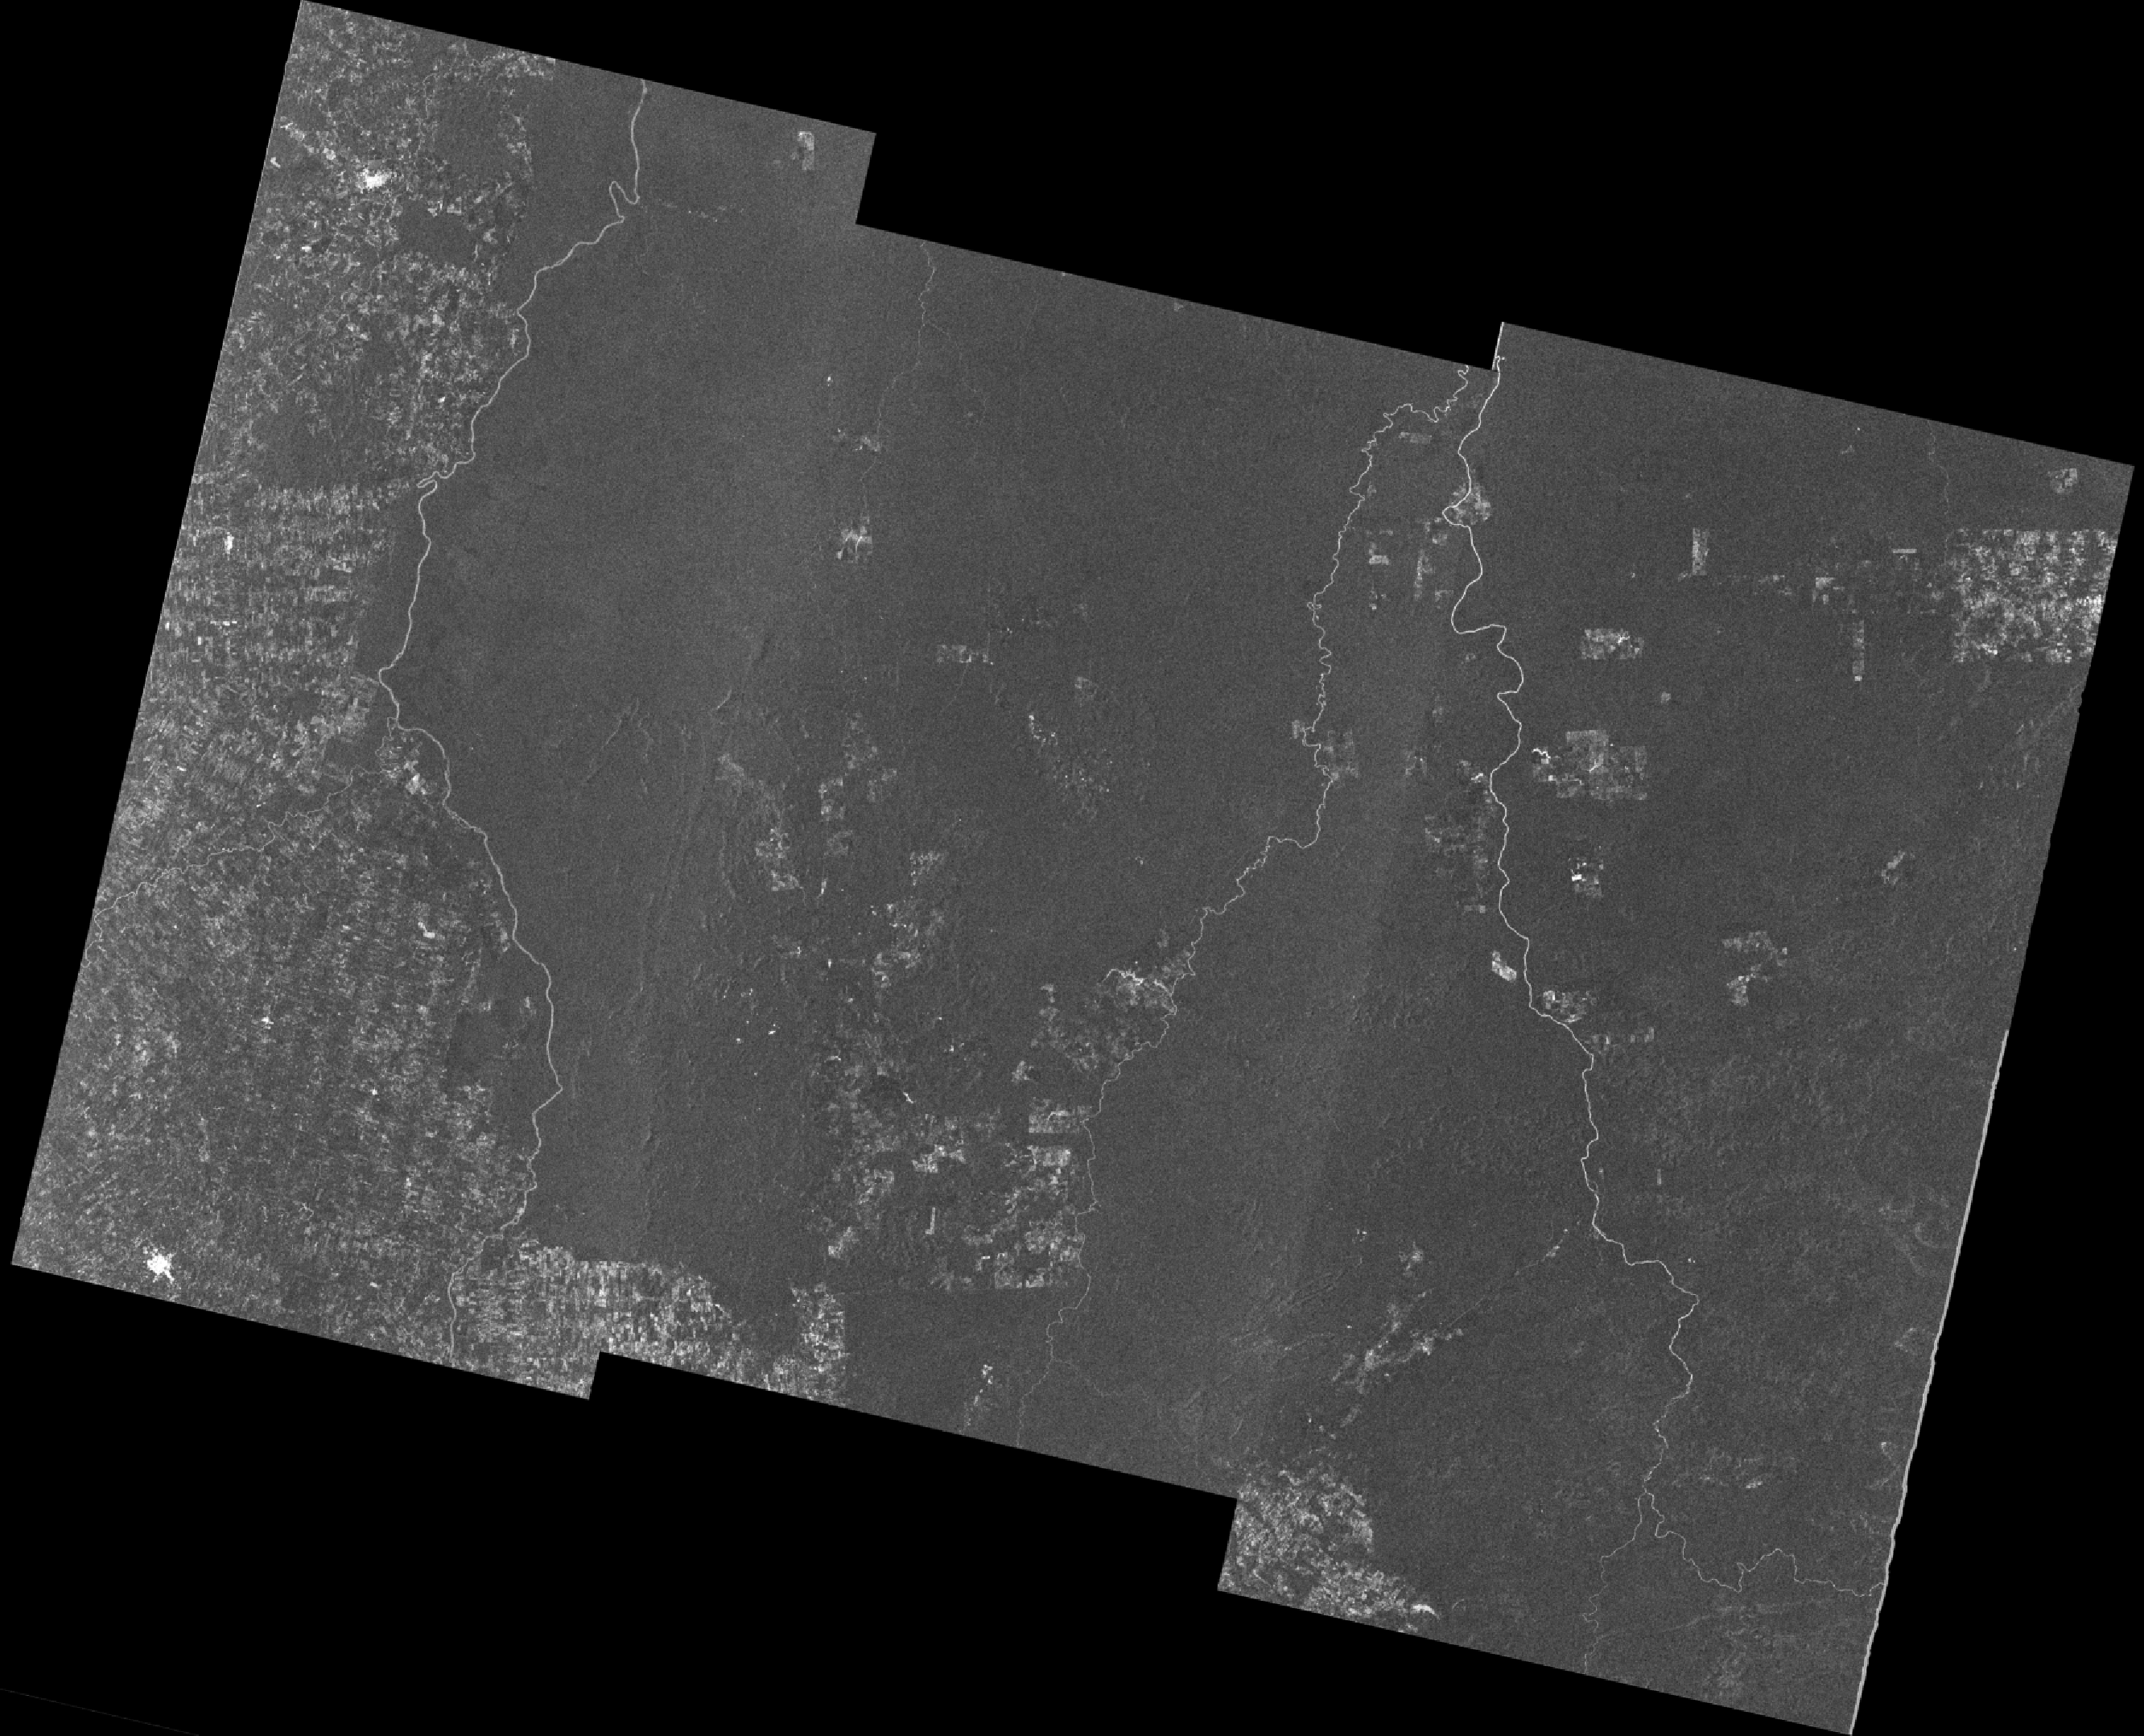
\includegraphics[width=0.75\linewidth]{Chapter5/SENTINEL1/geo_cohimage.pdf}
    \caption{$\gamma$ acquisition}
    \label{fig:gamma_sentinel}
\end{figure}{}
\begin{figure}[H]
    \centering
    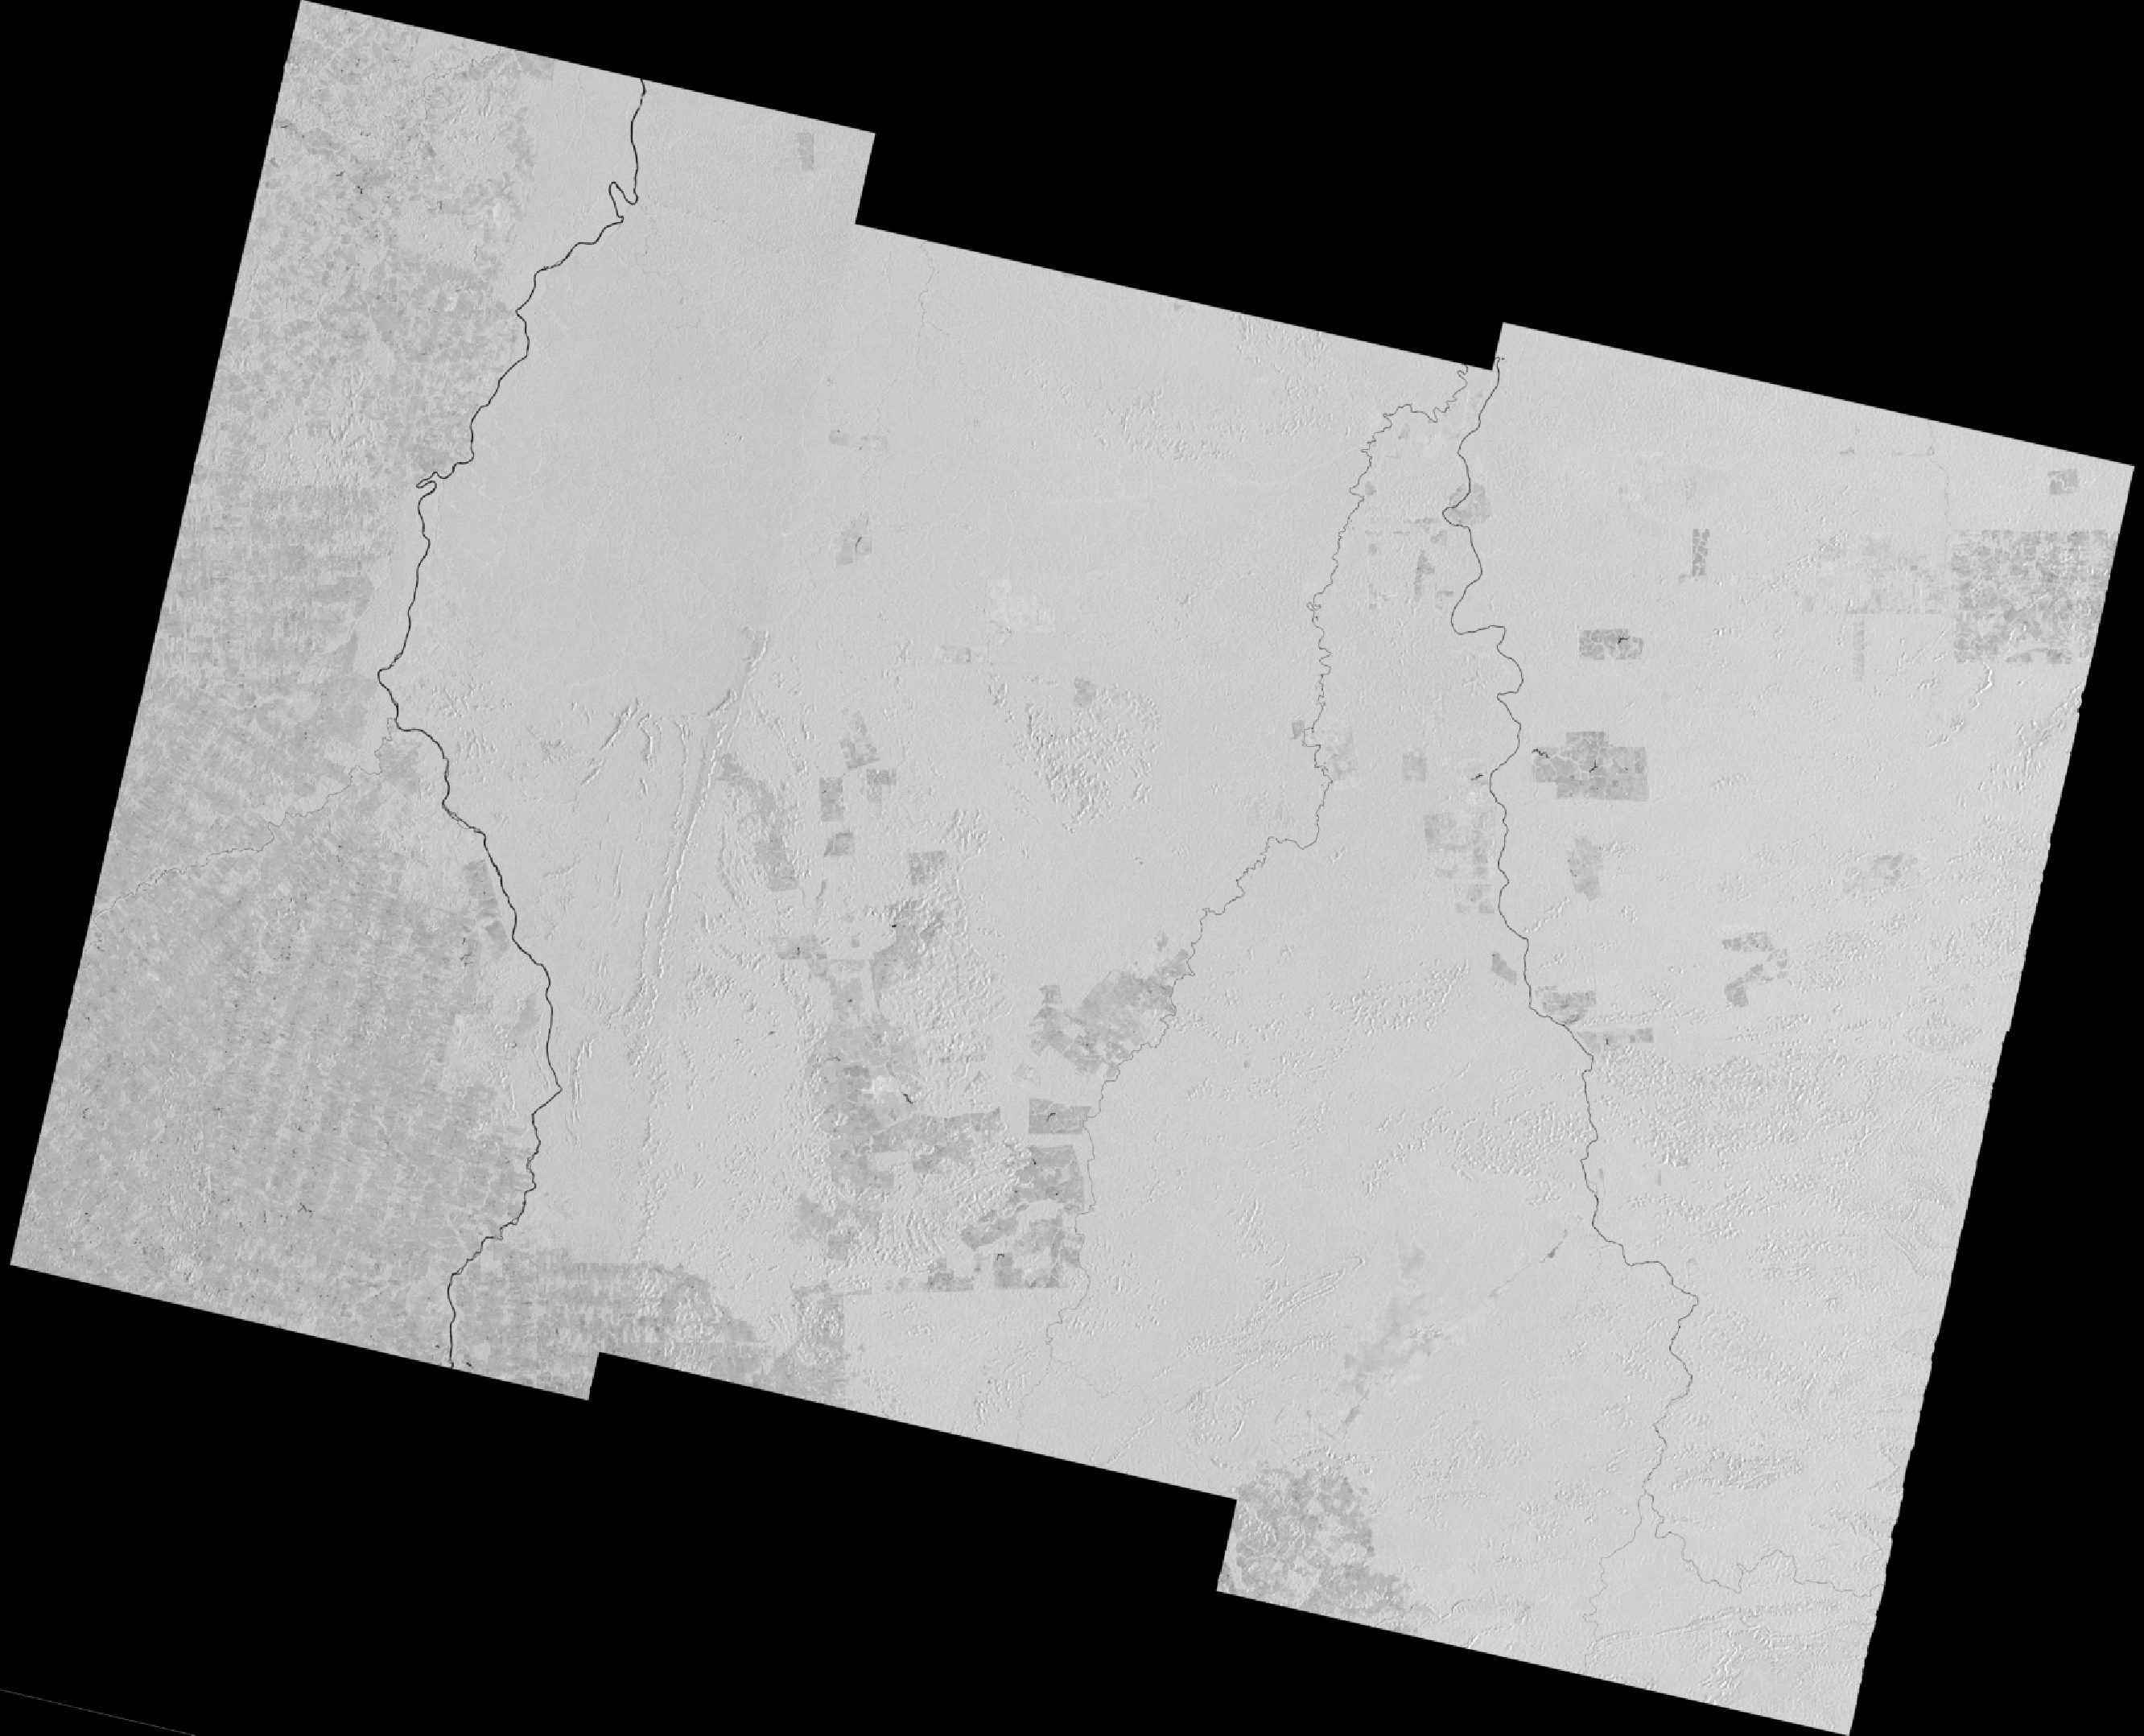
\includegraphics[width=0.75\linewidth]{Chapter5/SENTINEL1/geo_temp_sigma0dbimage.pdf}
    \caption{$\sigma^0$ acquisition}
    \label{fig:sigma_sentinel}
\end{figure}{}

\newpage
The respective histograms for the coherence and $\sigma^0$ can be seen below.

\begin{figure}[H]
  \centering
  \begin{subfigure}[b]{0.4\linewidth}
    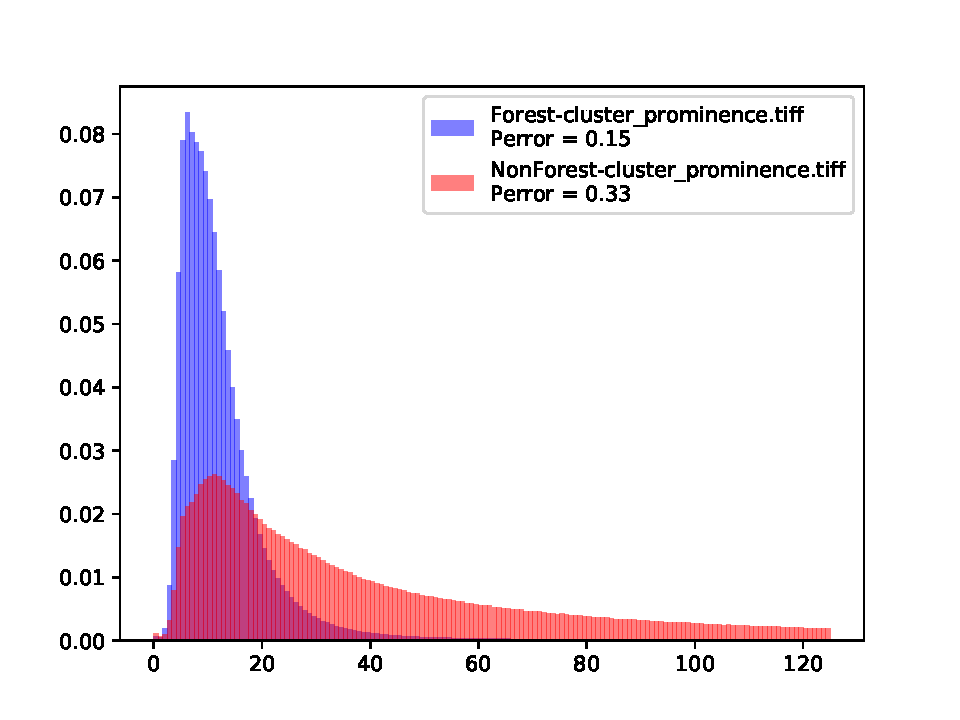
\includegraphics[width=\linewidth]{Chapter5/SENTINEL1/Coherence/cluster_prominence_histogram.pdf}
     \caption{Probability density Function for Cluster Prominence.}
  \end{subfigure}
  \centering
  \begin{subfigure}[b]{0.4\linewidth}
    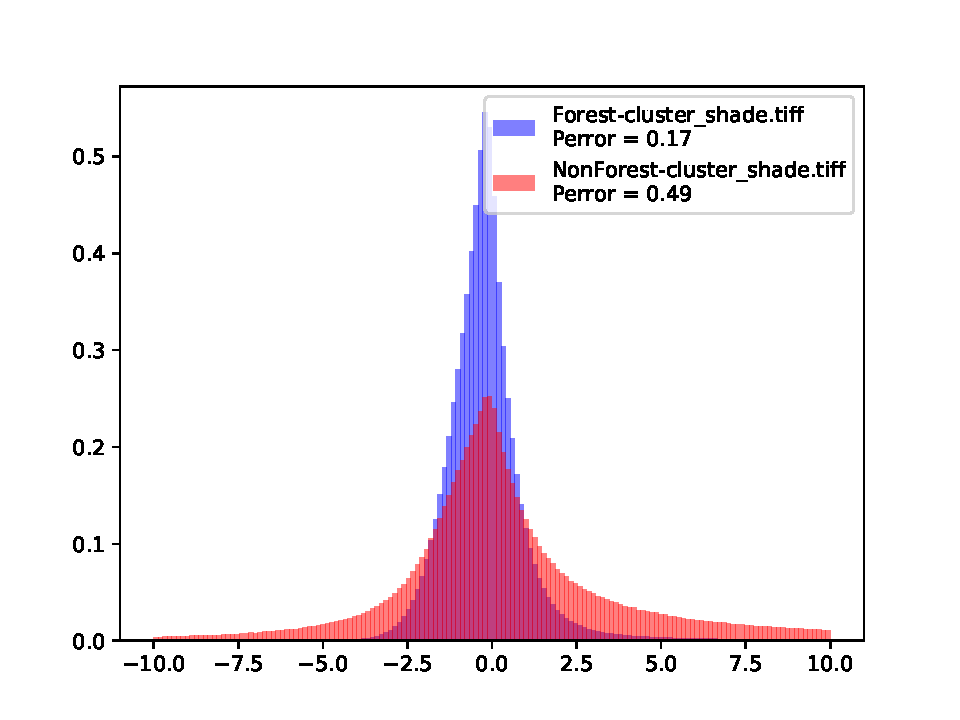
\includegraphics[width=\linewidth]{Chapter5/SENTINEL1/Coherence/cluster_shade_histogram.pdf}
     \caption{Probability density Function for Cluster Shade.}
  \end{subfigure}
  \centering
  \begin{subfigure}[b]{0.4\linewidth}
    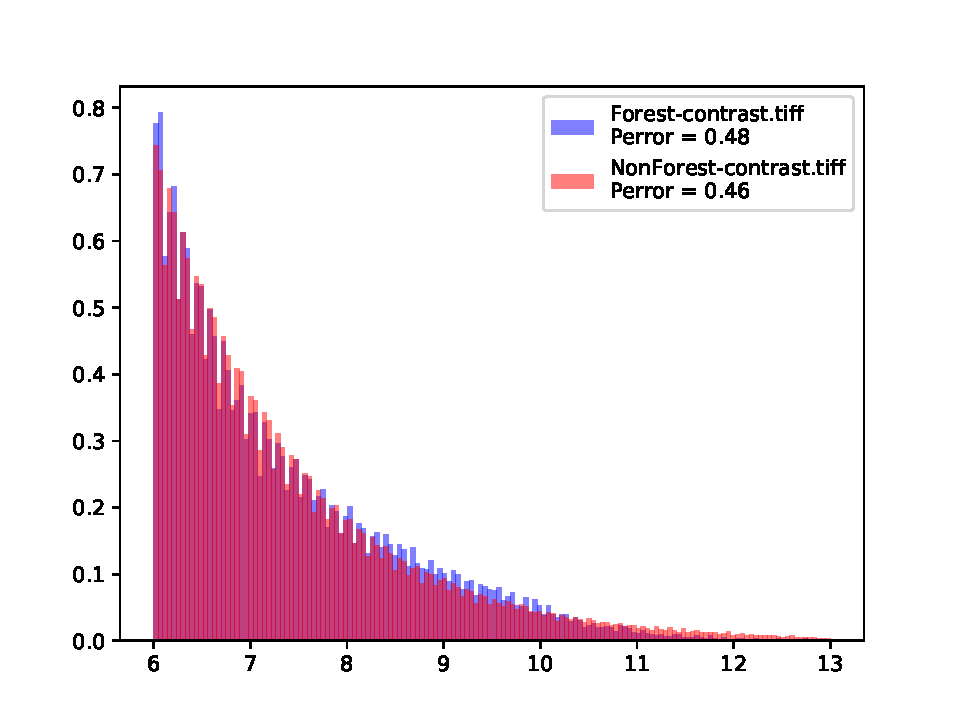
\includegraphics[width=\linewidth]{Chapter5/SENTINEL1/Coherence/contrast_histogram.pdf}
     \caption{Probability density Function for Contrast.}
  \end{subfigure}
  \centering
  \begin{subfigure}[b]{0.4\linewidth}
    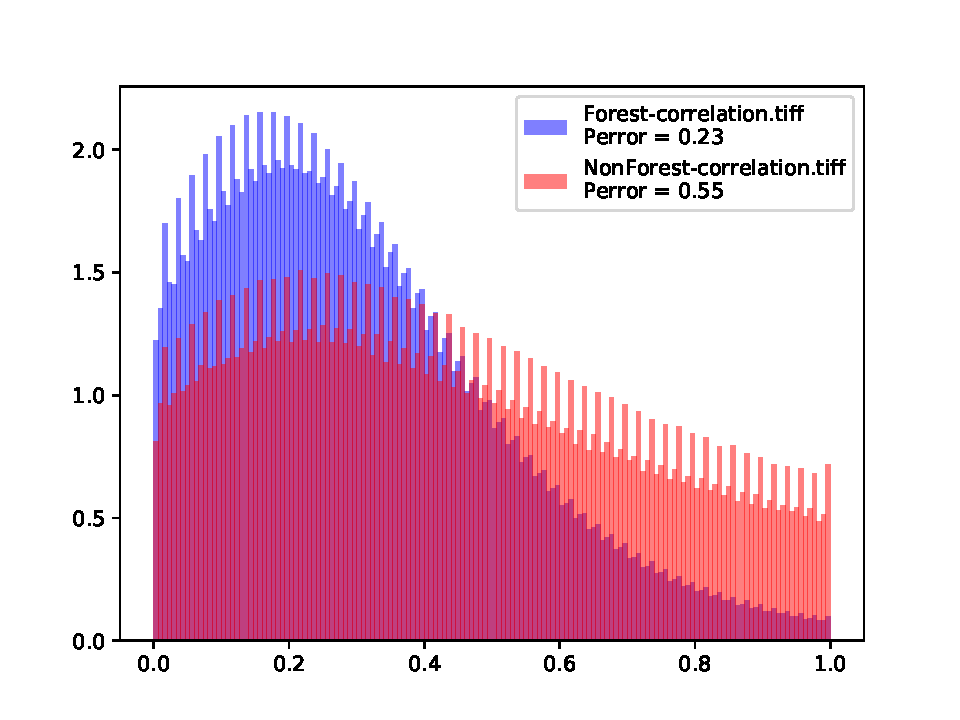
\includegraphics[width=\linewidth]{Chapter5/SENTINEL1/Coherence/correlation_histogram.pdf}
     \caption{Probability density Function for Correlation.}
  \end{subfigure}
  \centering
  \begin{subfigure}[b]{0.4\linewidth}
    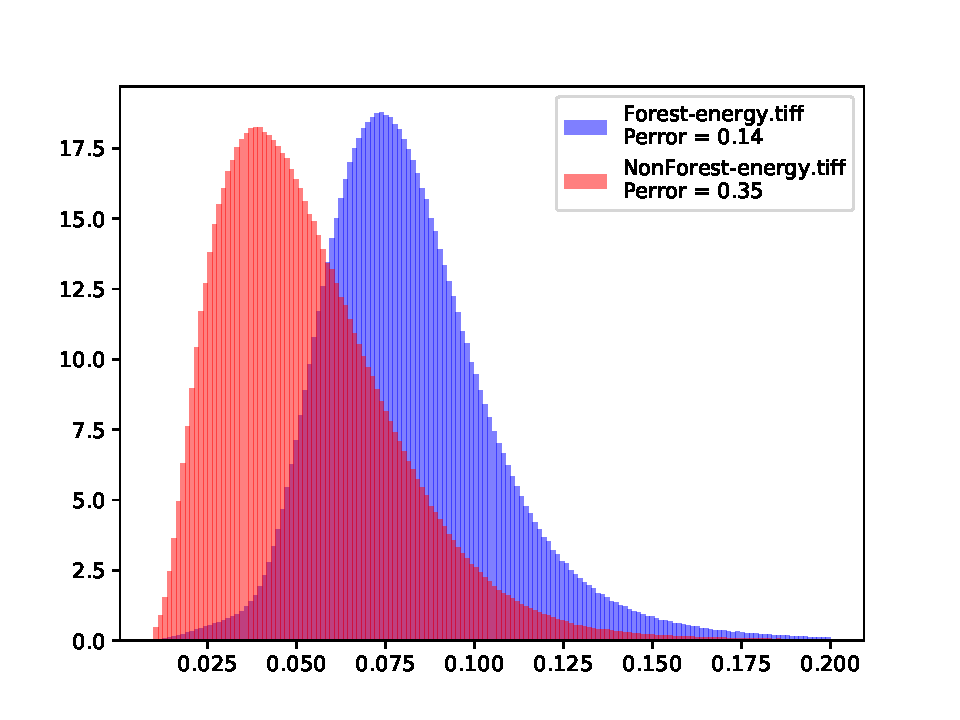
\includegraphics[width=\linewidth]{Chapter5/SENTINEL1/Coherence/energy_histogram.pdf}
     \caption{Probability density Function for Energy.}
  \end{subfigure}
  \centering
  \begin{subfigure}[b]{0.4\linewidth}
    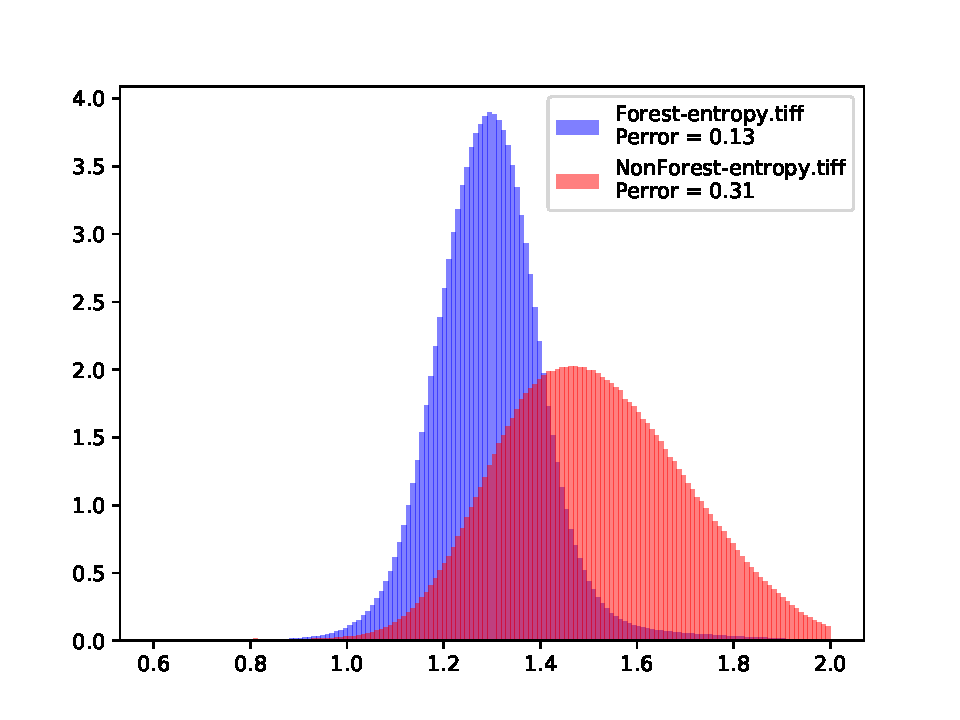
\includegraphics[width=\linewidth]{Chapter5/SENTINEL1/Coherence/entropy_histogram.pdf}
     \caption{Probability density Function for Entropy.}
  \end{subfigure}
\end{figure}

\begin{figure}[H]\ContinuedFloat
  \centering
  \begin{subfigure}[b]{0.4\linewidth}
    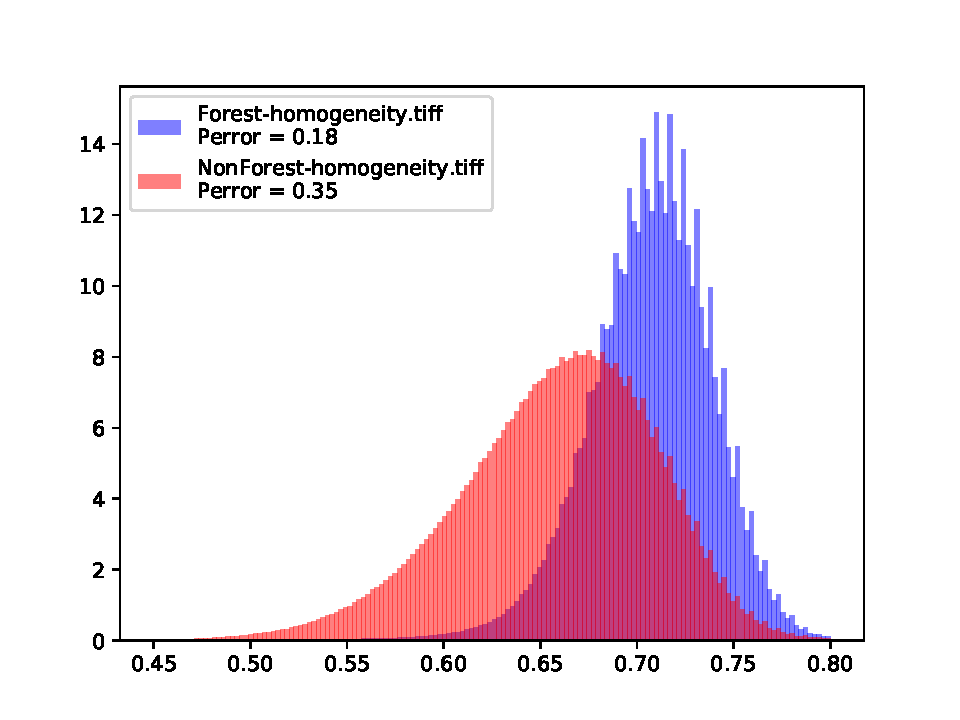
\includegraphics[width=\linewidth]{Chapter5/SENTINEL1/Coherence/homogeneity_histogram.pdf}
     \caption{Probability density Function for Homogeneity.}
  \end{subfigure}
  
  \centering
  \begin{subfigure}[b]{0.4\linewidth}
    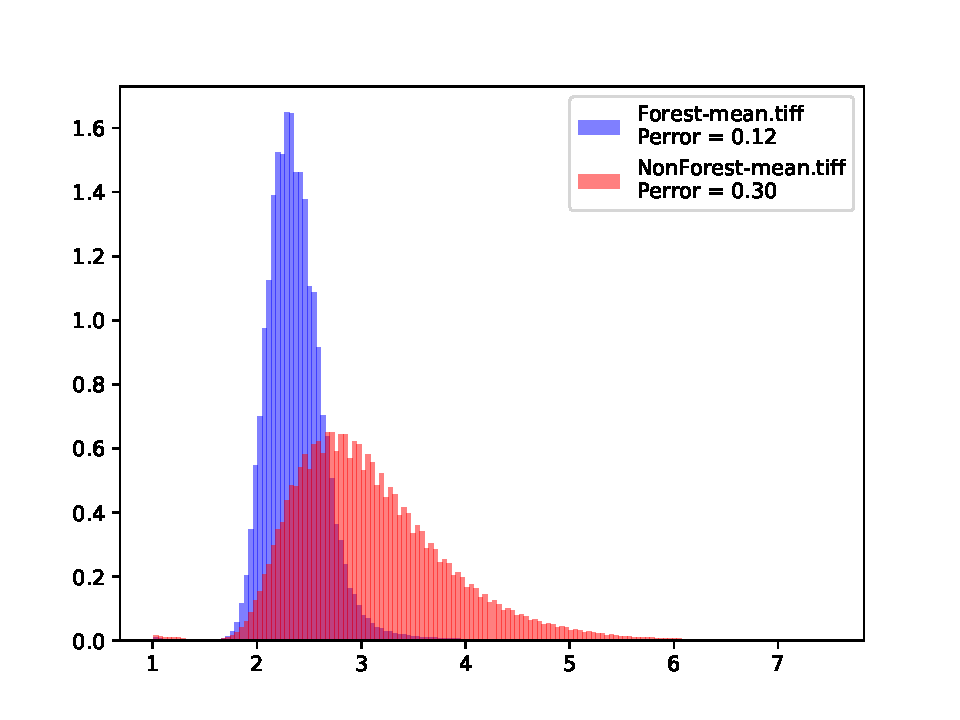
\includegraphics[width=\linewidth]{Chapter5/SENTINEL1/Coherence/mean_histogram.pdf}
     \caption{Probability density Function for Mean.}
  \end{subfigure}
  
  \centering
  \begin{subfigure}[b]{0.4\linewidth}
    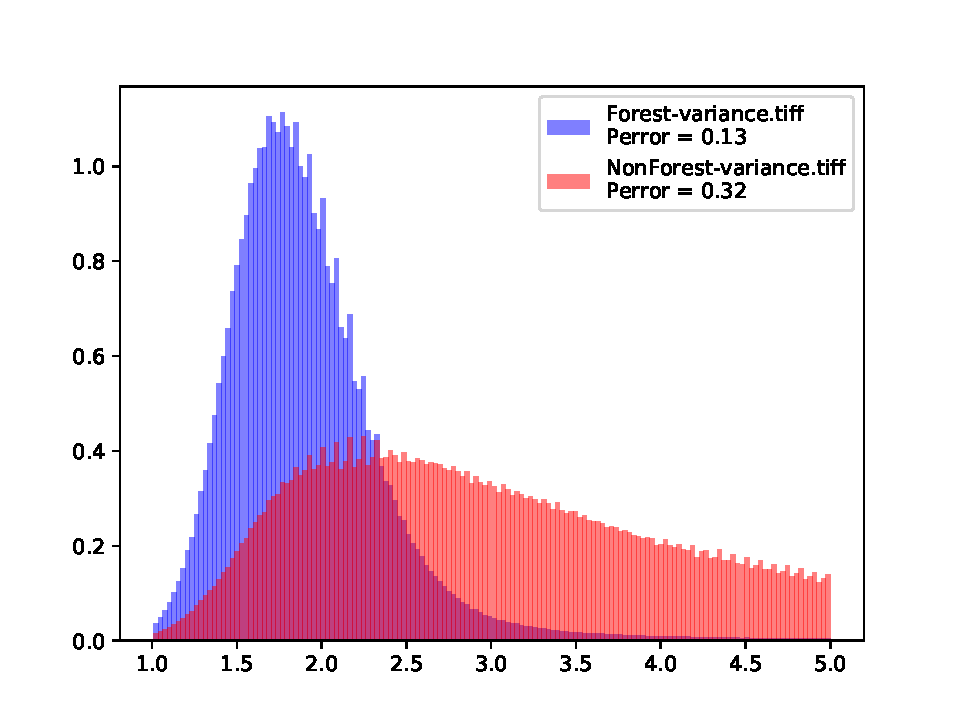
\includegraphics[width=\linewidth]{Chapter5/SENTINEL1/Coherence/variance_histogram.pdf}
     \caption{Probability density Function for Variance.}
  \end{subfigure}
  \caption{Histograms of Coherence Textures}
  \label{fig: sentinel_coherence_hist}
\end{figure}
\newpage


\begin{figure}[H]
  \centering
  \begin{subfigure}[b]{0.4\linewidth}
    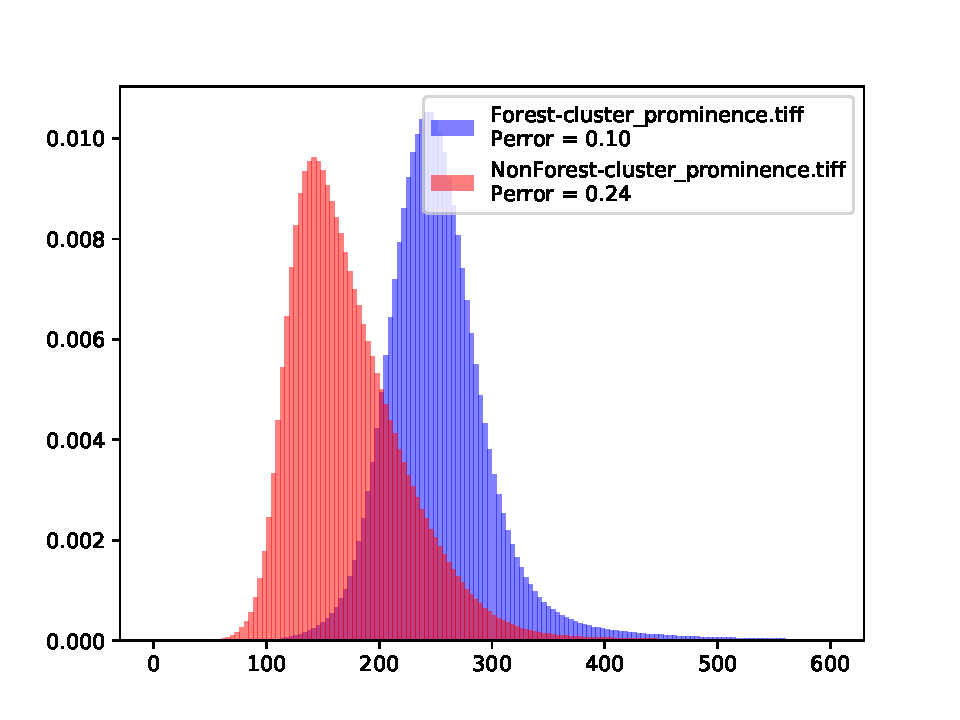
\includegraphics[width=\linewidth]{Chapter5/SENTINEL1/Sigma0/cluster_prominence_histogram.pdf}
     \caption{Probability density Function for Cluster Prominence.}
  \end{subfigure}
  \centering
  \begin{subfigure}[b]{0.4\linewidth}
    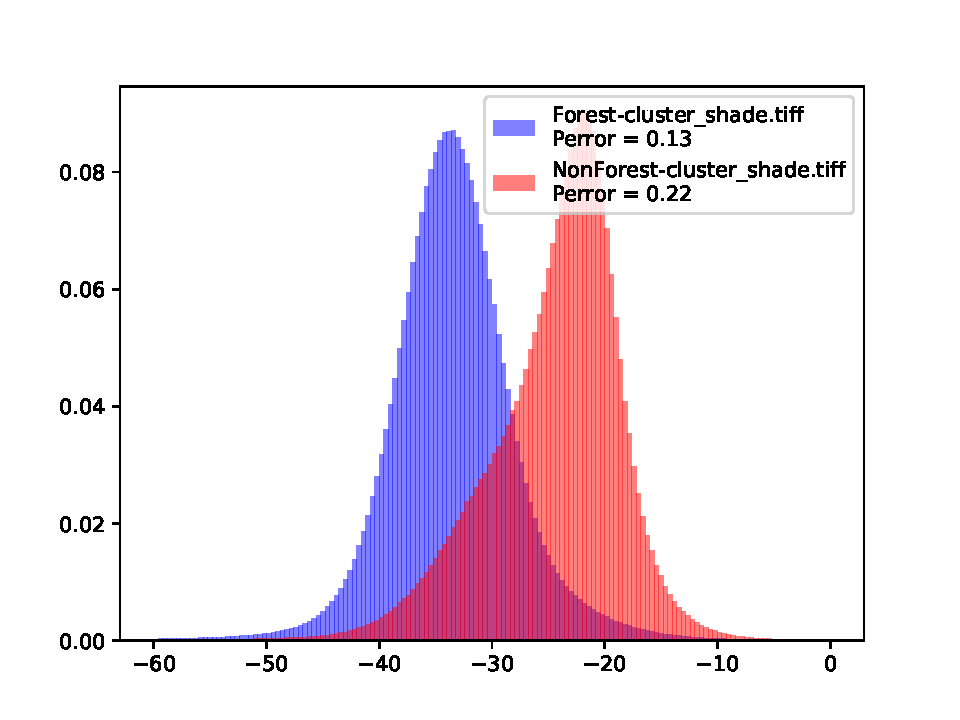
\includegraphics[width=\linewidth]{Chapter5/SENTINEL1/Sigma0/cluster_shade_histogram.pdf}
     \caption{Probability density Function for Cluster Shade.}
  \end{subfigure}
  \centering
  \begin{subfigure}[b]{0.4\linewidth}
    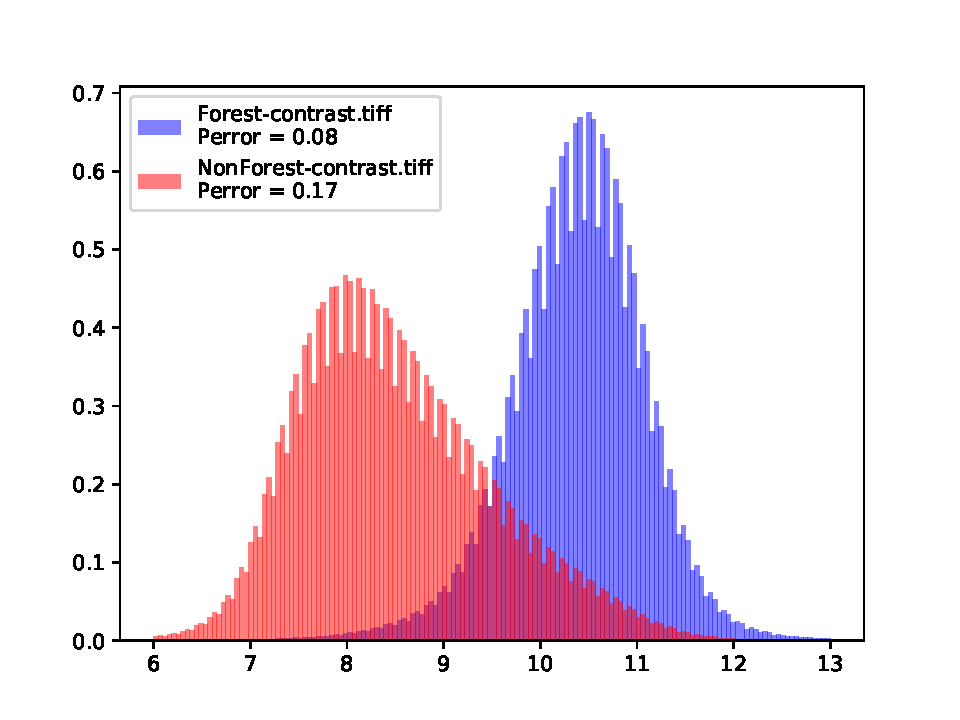
\includegraphics[width=\linewidth]{Chapter5/SENTINEL1/Sigma0/contrast_histogram.pdf}
     \caption{Probability density Function for Contrast.}
  \end{subfigure}
  \centering
  \begin{subfigure}[b]{0.4\linewidth}
    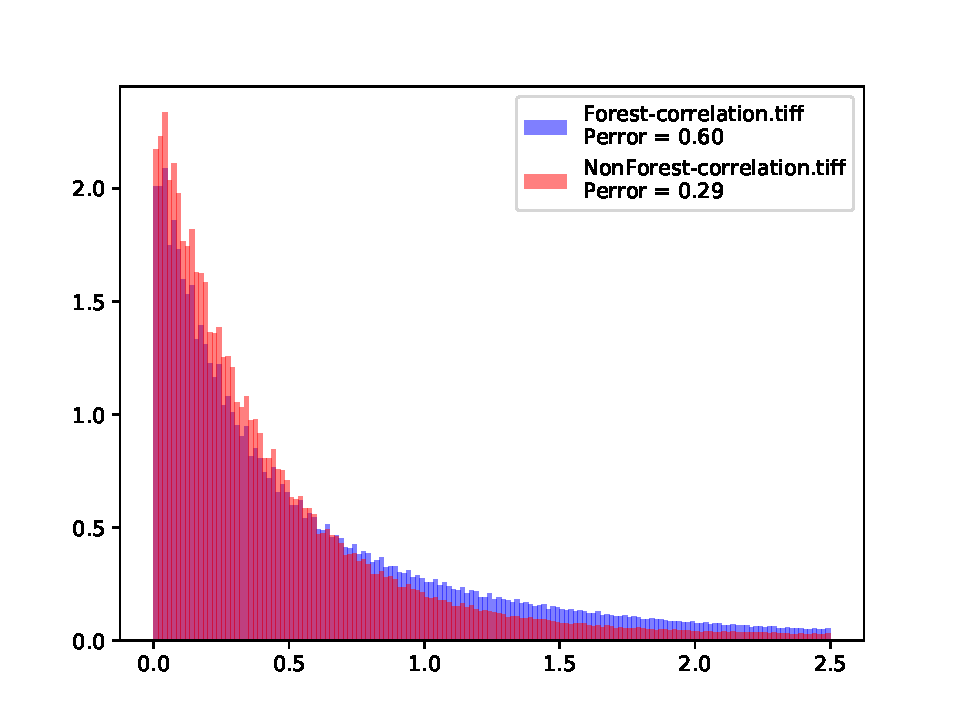
\includegraphics[width=\linewidth]{Chapter5/SENTINEL1/Sigma0/correlation_histogram.pdf}
     \caption{Probability density Function for Correlation.}
  \end{subfigure}
  \centering
  \begin{subfigure}[b]{0.4\linewidth}
    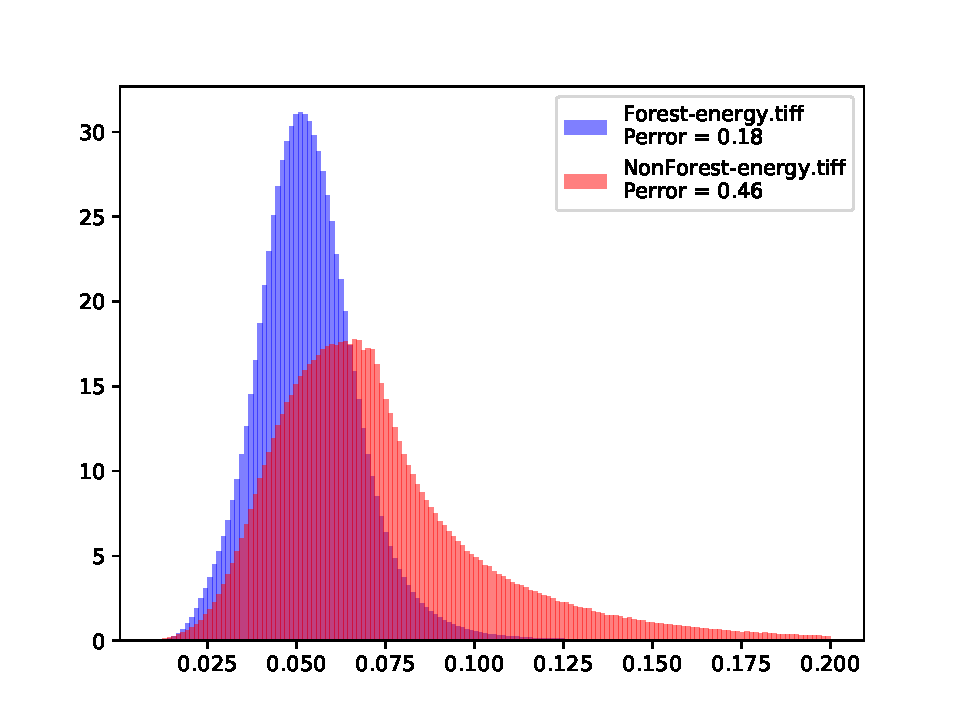
\includegraphics[width=\linewidth]{Chapter5/SENTINEL1/Sigma0/energy_histogram.pdf}
     \caption{Probability density Function for Energy.}
  \end{subfigure}
  \centering
  \begin{subfigure}[b]{0.4\linewidth}
    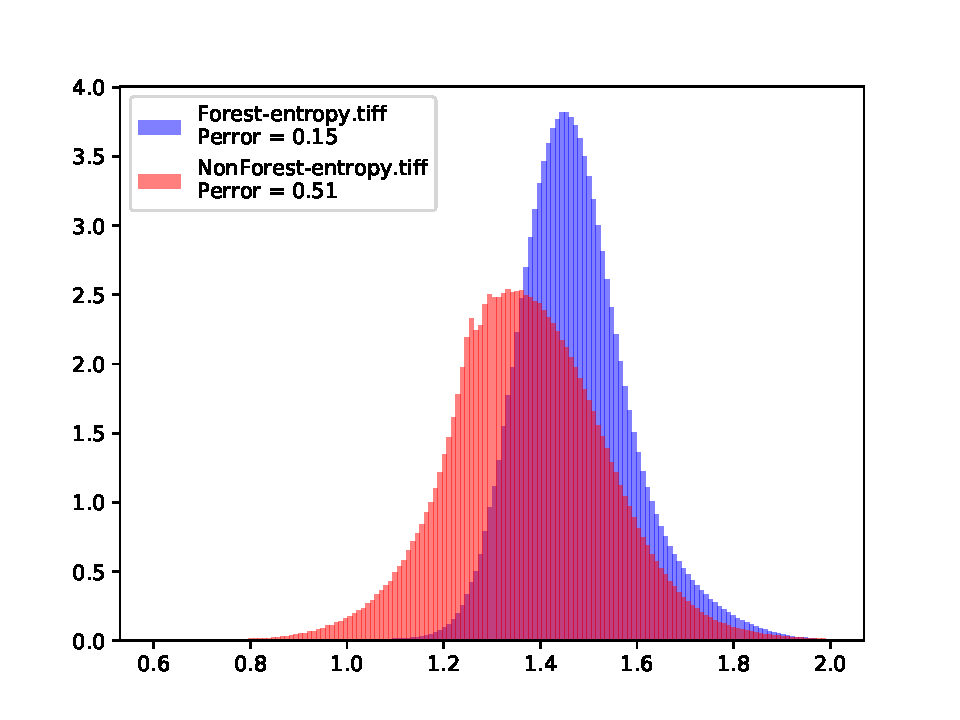
\includegraphics[width=\linewidth]{Chapter5/SENTINEL1/Sigma0/entropy_histogram.pdf}
     \caption{Probability density Function for Entropy.}
  \end{subfigure}
  \centering
\end{figure}

\begin{figure}[H]\ContinuedFloat
    \centering
    \begin{subfigure}[b]{0.4\linewidth}
        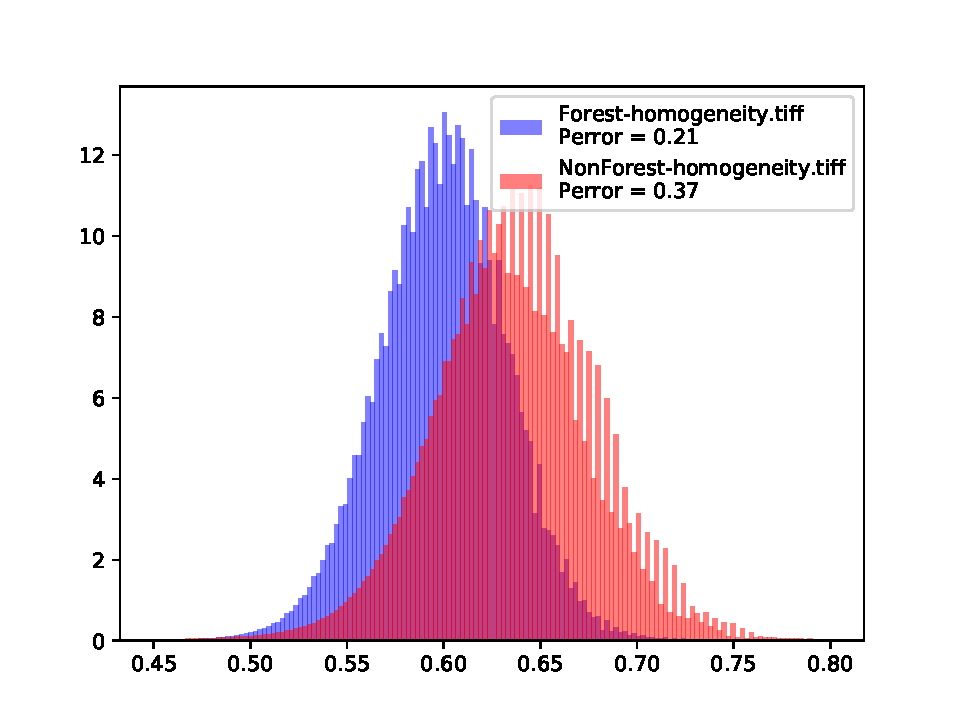
\includegraphics[width=\linewidth]{Chapter5/SENTINEL1/Sigma0/homogeneity_histogram.pdf}
        \caption{Probability density Function for Homogeneity.}
    \end{subfigure}
  
  \centering
  \begin{subfigure}[b]{0.4\linewidth}
    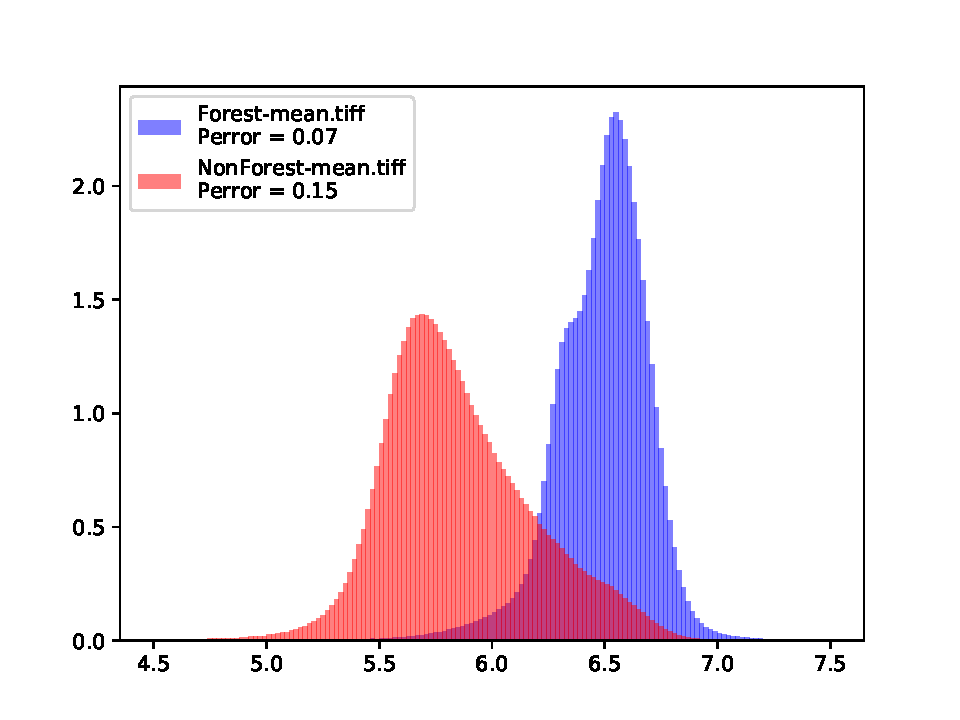
\includegraphics[width=\linewidth]{Chapter5/SENTINEL1/Sigma0/mean_histogram.pdf}
    \caption{Probability density Function for Mean.}
  \end{subfigure}
  \centering

    \centering
    \begin{subfigure}[b]{0.4\linewidth}
        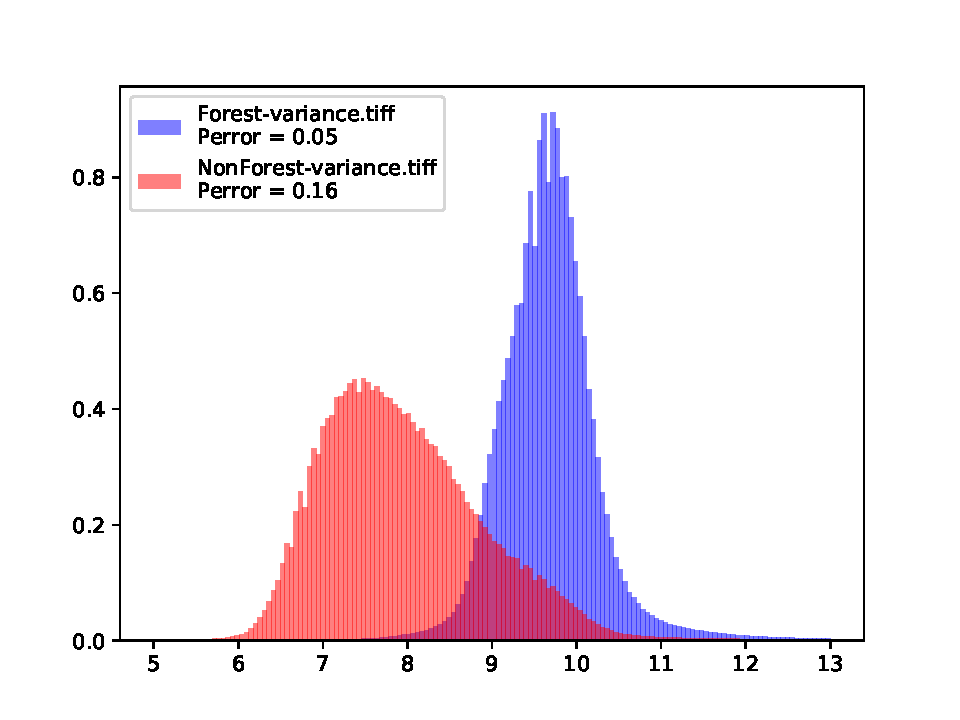
\includegraphics[width=\linewidth]{Chapter5/SENTINEL1/Sigma0/variance_histogram.pdf}
        \caption{Probability density Function for Variance.}
        \end{subfigure}
    \caption{Histograms of $\sigma^0$ Textures}
    \label{fig: sentinel_sigma_hist}
\end{figure}

From the images and the histograms above it is clear that it is harder to make a classification, as the $\sigma^0$ and $\gamma$ are not as separated as TANDEM-X acquisition.
\begin{figure}[H]
    \centering
    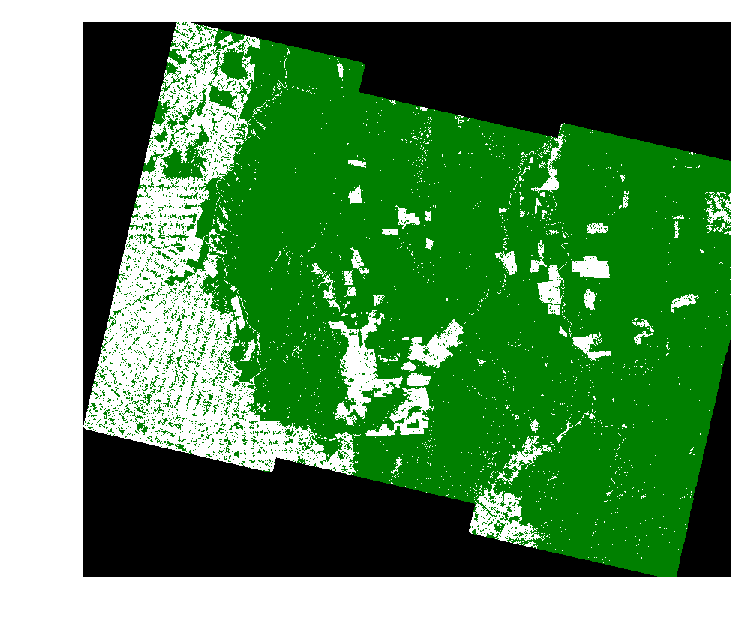
\includegraphics[width=\linewidth]{Chapter5/TANDEM-X/reference_mapimage.pdf}
    \caption{Reference Map provided by DLR}
    \label{fig:ref_sentinel}
\end{figure}{}

Below it is possible to see the classification result using only the coherence and the $\sigma^0$ as input to the random forest.
\begin{figure}[H]
    \centering
    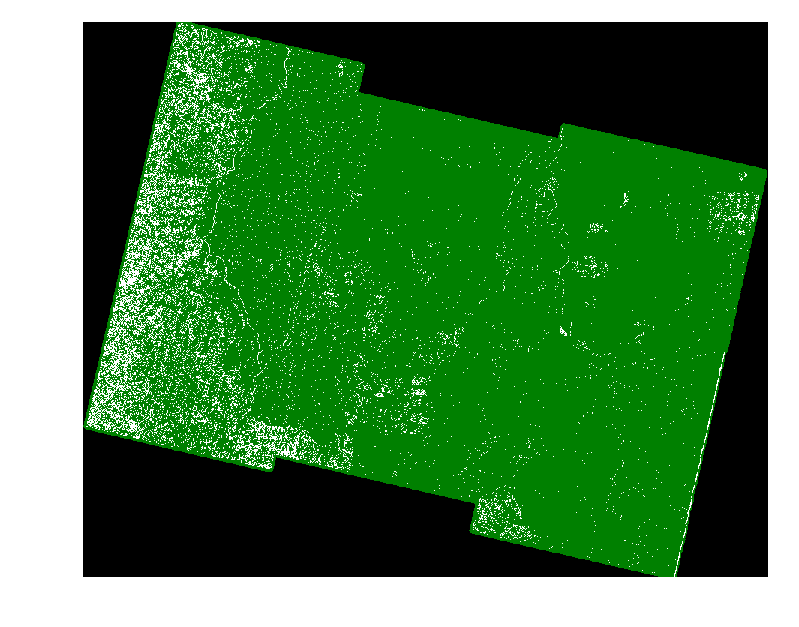
\includegraphics[width=\linewidth]{Chapter5/TANDEM-X/result_no_texturesimage.pdf}
    \caption{Classification Results without textures}
    \label{fig:result_no_textures_sentinel}
\end{figure}{}
It is clear from that image the limitations of the machine learning algorithms for classification, since the classification clearly has a low accuracy. Below it is possible to see the random forest result using the textures.

\begin{figure}[H]
    \centering
    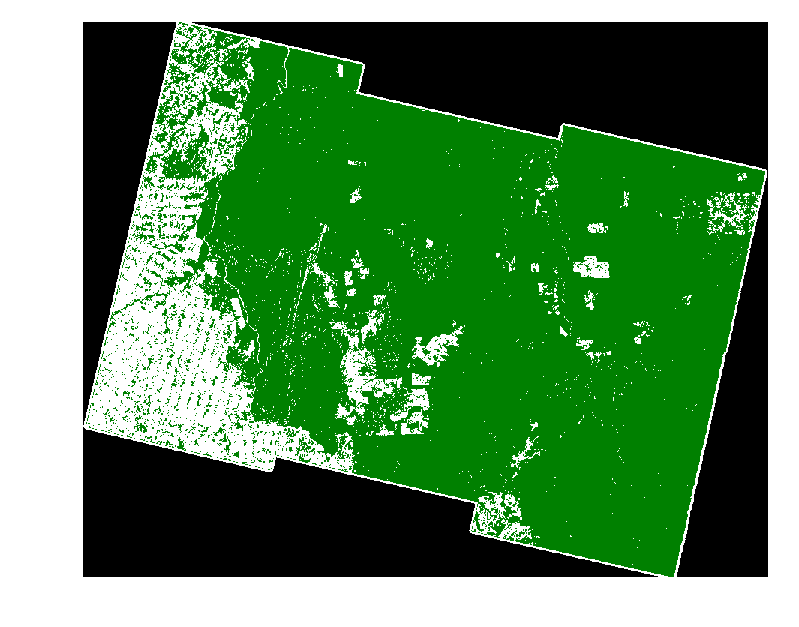
\includegraphics[width=\linewidth]{Chapter5/TANDEM-X/result_texturesimage.pdf}
    \caption{Classification Results with textures}
    \label{fig:result_textures_sentinel}
\end{figure}{}

From that new image it is now clear how powerful the textures can be in aiding classification algorithms.
For comparison, below it is also attached the optical image of the area acquired via Google Earth. The area acquired with Sentinel1 is show in the red square.

\begin{figure}[H]
    \centering
    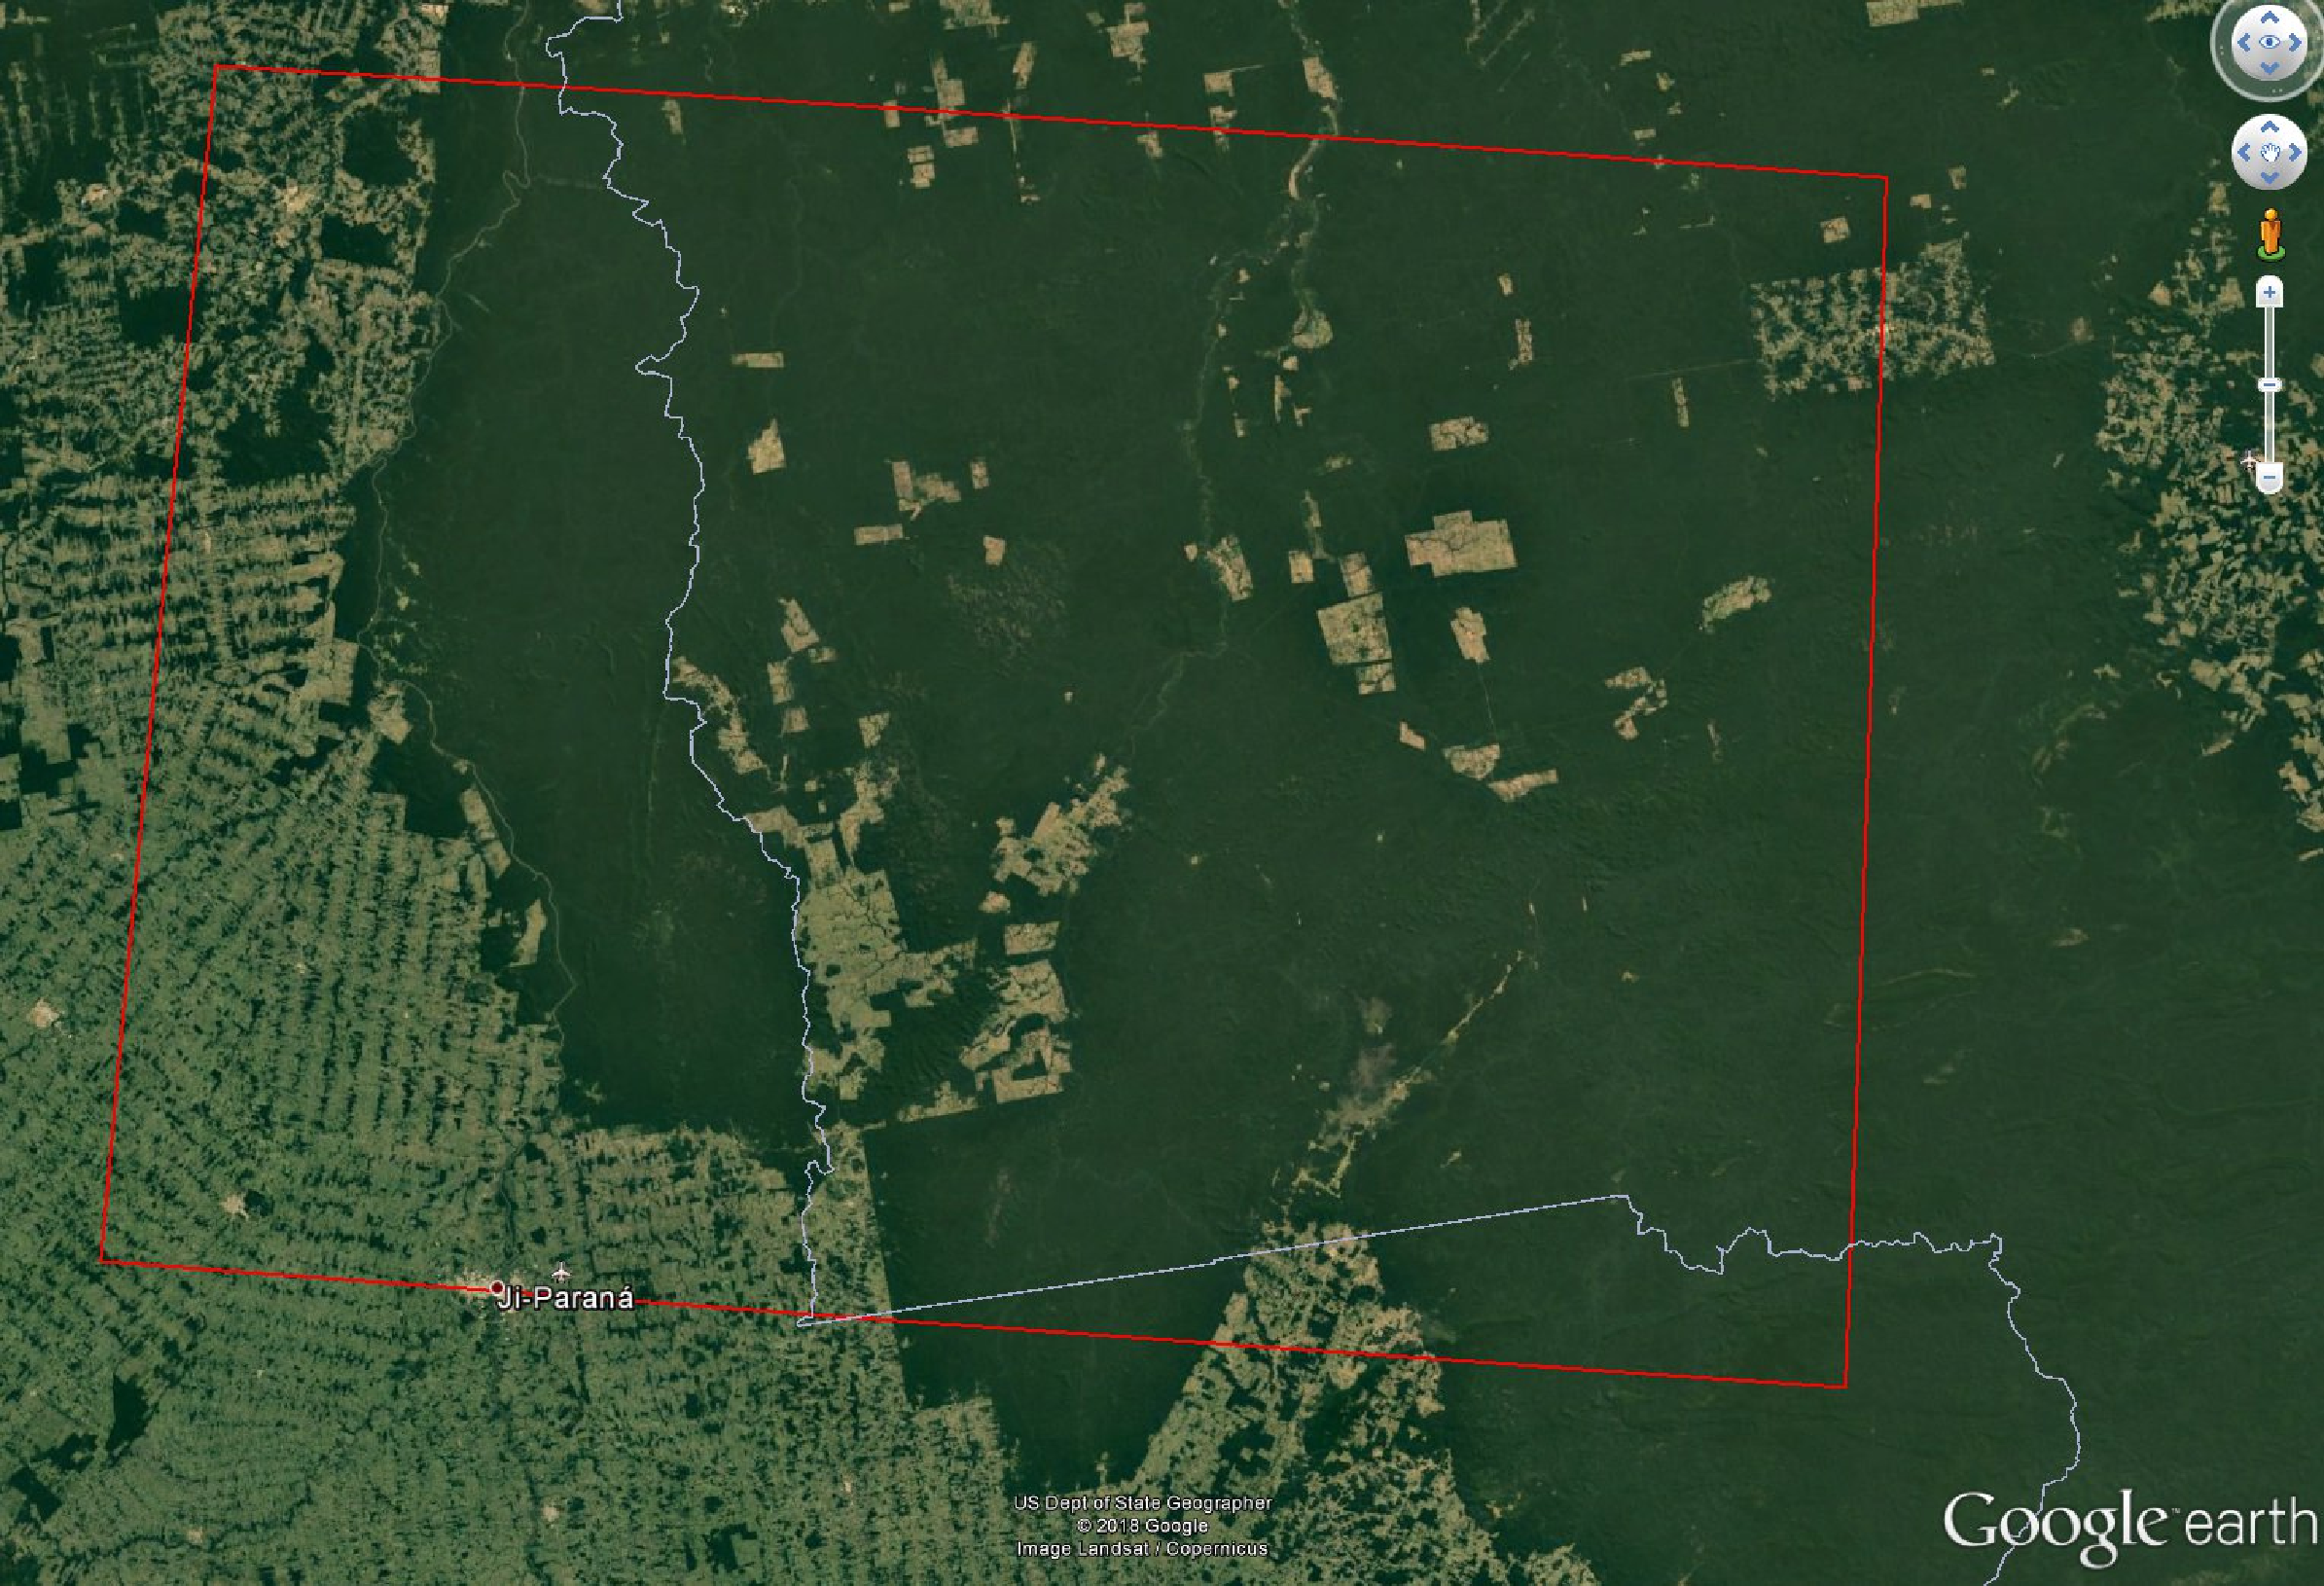
\includegraphics[width=\linewidth]{Chapter5/real_image_google_earth.pdf}
    \caption{Google Earth image of analysed area}
    \label{fig:google_earth_area_sentinel1}
\end{figure}{}

\section{Performance of Random forest and parameters tuning}
There are 3 important parameters that have great impact on the performance of the Random Forest algorithm:
\begin{itemize}
    \item Number of estimators: The number of trees in the forest.
    \item Maximum depth: The maximum depth of the tree
    \item Minimum samples for leaf: The minimum number of samples required to be at a leaf node. A split point at any depth will only be considered if it leaves at the minimum number of samples for leaf training samples in each of the left and right branches
\end{itemize}{}

Even though increasing those parameters can lead to greater accuracy, there are some breaking points in which the accuracy decreases, and there are some points in which the accuracy is stagnated and will not further increase, therefore only wasting computational time for no valuable return. For example, one might think that increasing the depth of the tree would yield a greater accuracy, but there is a limit in which the results will not improve, but it will take more time for the algorithm to make the training and the classification.
Below there area images that show how the accuracy of the classification algorithm changes with variations on the parameters:
\begin{figure}[H]
    \centering
    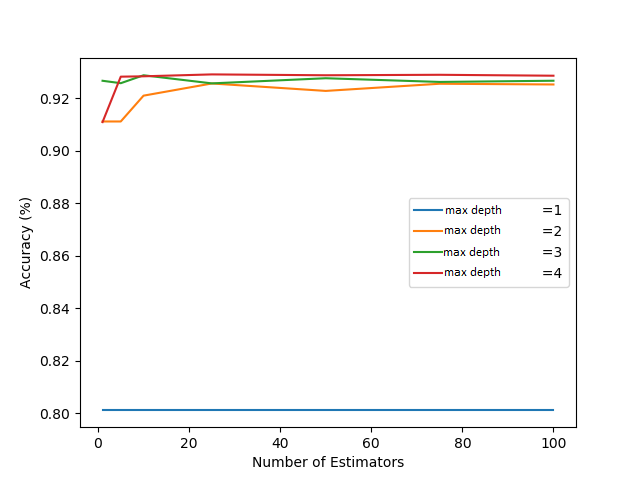
\includegraphics[width=\linewidth]{Chapter5/Number_of_estimators.png}
    \caption{Accuracy versus number of estimators for different tree depths}
    \label{fig:num_estimators}
\end{figure}{}

\begin{figure}[H]
    \centering
    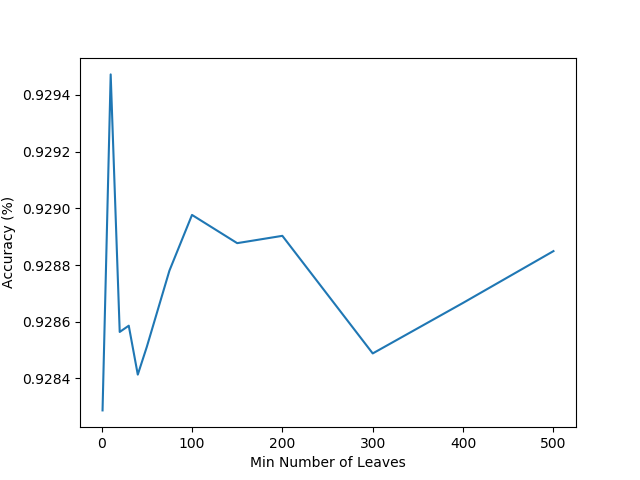
\includegraphics[width=\linewidth]{Chapter5/number_of_leaves.png}
    \caption{Accuracy versus minimum number of samples for leaf parameter}
    \label{fig:num_leaves}
\end{figure}{}
